\documentclass[12pt]{iopart}
\bibliographystyle{iopart-num}

\usepackage{hyperref}
\usepackage[numbers,sort&compress]{natbib}
\usepackage{hypernat}
\usepackage{graphicx}
\graphicspath{ {Figures/} }
\usepackage{multirow}
\usepackage{subcaption}
\usepackage{array}

\begin{document}

\title[Link between divertor conditions and HFS/LFS midplane density profiles in H-mode plasmas at ASDEX Upgrade]{Link between divertor conditions and HFS/LFS midplane density profiles in H-mode plasmas at ASDEX Upgrade}
\author{L. Guimarais$^1$, C. Silva$^1$, M. Bernert$^2$, G. D. Conway$^2$, A. Drenik$^2$, L. Gil$^1$, V. Nikolaeva$^{1}$, T. Reichbauer$^2$, F. Reimold$^3$, J. Santos$^1$, E. Seliunin$^1$, A. Silva$^1$, U. Stroth$^{2,4}$, J. Vicente$^1$, E. Wolfrum$^2$, the ASDEX Upgrade Team and the EUROfusion MST1 team$^*$}

\address{$^1$ Instituto de Plasmas e Fus\~ao Nuclear, Instituto Superior T\'ecnico, Universidade de Lisboa, Portugal}
\address{$^2$ Max-Planck-Institut f\"ur Plasmaphysik, Boltzmannstr. 2, 85748, Garching, Germany}
\address{$^3$ Forschungszentrum J\"ulich GmbH, Wilhelm-Johnen-Stra{\ss}e, 52425 J\"ulich, Germany}
\address{Physik-Department E28, Technische Universit\"at M\"unchen, James-Franck-Str. 1, 85748 Garching, Germany}
\begin{center}
\address{$^*$ 
%See \url{http://www.euro-fusionscipub.org/mst1}}
See the author list of Meyer et al, Overview of progress in European Medium Sized Tokamaks towards an integrated plasma-edge/wall solution, accepted for publication in Nuclear Fusion}
\end{center}

\ead{guimas@ipfn.tecnico.ulisboa.pt}
\vspace{10pt}
\begin{indented}
\item[]Somewhen 2018
\end{indented}

%%%%%%%%%%%%%%%%%%%%%%%%%%%%%%%%%%%%%%%%%%%%%%%%%%%%%%%%%%%%%%%%
\begin{abstract}
\label{sec:abstract}

The connection between midplane and divertor conditions is studied on ASDEX Upgrade for H-mode. H-mode discharges are analysed where fuelling, heating power and impurity seeding are scanned, enabling to disentangle their role on the evolution of LFS/HFS midplane density profiles. The high resolution High-Field-Side (HFS) / Low-Field-Side (LFS) O-mode reflectometer provides a unique insight into plasma conditions at both the in- and outboard side. At the inner divertor, with the onset of detachment, a region of high density is formed (High Field Side High Density front, HFSHD) and it is seen to expand into the HFS midplane. The evolution of HFS midplane density profiles strongly responds to the state of the inner divertor and to the presence of the HFSHD. At the LFS, the density profile at the SOL is also greatly correlated with divertor conditions, providing further evidence to previous observations. Fast transient events (Edge Localised Modes, ELMs) are a feature of the H-mode, which complicate the analysis. The interplay between midplanes and divertors is separately analysed for the inter-ELM period and then for the ELM cycle itself. 
\end{abstract}

%%%%%%%%%%%%%%%%%%%%%%%%%%%%%%%%%%%%%%%%%%%%%%%%%%%%%%%%%%%%%%%%
\section{Introduction}
\label{sec:intro}

H-mode occurs above a threshold heating power and leads to the formation of an edge transport barrier that is associated with the increase of electron density and temperature in the pedestal region\cite{wagner1982regime}. The higher heating power necessary to sustain H-modes also requires a higher density for detachment\cite{LaBombard1987,krasheninnikov1998physical} to arise. In ASDEX Upgrade (AUG), with a tungsten (W) wall, only a partially detached outer target has been achieved in non-seeded H-mode. When gas fuelling is applied at sufficient heating power, a poloidally localised region of high density at the HFS SOL appears, at the height of the X-point, the so called High Field Side High Density front (HFSHD). The HFSHD is found in L- and H-mode plasmas and has so far been observed on AUG\cite{mccormick2009main,Potzel2015} and JET\cite{potzel2015formation} revealing that the presence of a HFSHD is independent of confinement mode and machine size. Typically, the HFSHD has a density one order of magnitude larger than that at the separatrix. The HFSHD is associated with the detachment of the inner divertor while the outer divertor may be attached or detached and found to be correlated with neutral fluxes in the far SOL as both increase with heating power\cite{Reimold2015}. The magnitude of the HFSHD is reduced or even suppressed with impurity seeding due to the radiation of the exhausted power before it reaches the HFS SOL preventing the ionisation of particles associated with the HFSHD\cite{potzel2015formation}. However, even at high N seeding fractions, it is not possible at AUG to completely mitigate the HFSHD. It was also suggested that nitrogen seeding in machines with metallic plasma facing components acts like the intrinsic radiator in carbon machines\cite{potzel2015formation}, thus explaining the rare observations of the HFSHD in non-metallic wall devices\cite{mccormick2009main}. 

The H-mode is foreseen as the standard operational scenario of future fusion devices such as ITER. Unfortunately, there are conflicting interests when it comes to achieve high-performance plasma conditions and how to handle their particle and power exhaust. Performance benefits from having large density gradients at the edge, close to the separatrix\cite{schneider2014pedestal}. On the other hand, plasma exhaust benefits from high edge densities\cite{kallenbach2018parameter}. The density at the separatrix is, therefore, an important interface parameter between the plasma core (performance) and the plasma edge (exhaust). In this work, we will explore how the LFS/HFS reflectometer can contribute to the interplay between performance and exhaust.

The confinement quality of a discharge is described by the factor $H_{98}$ that compares the achieved confinement to the prediction of the $H_{98,y2}$\cite{ITER1999} scaling (standard H-mode confinement corresponds to $H_{98} = 1$). The $H_{98}$ factor ranges from 0.8 to 1.2 in our experiments. Divertor detachment appears as an attractive scenario to handle power and particle loads, as their mitigation is fundamental for the integrity of Plasma Facing Components (PFCs).
%A power threshold of $10\,MW/m^{2}$ is defined as the engineering limit for PFCs for future devices.

This paper is organised as follows: section \ref{section:descriptionhmode} presents a description of the H-mode experiments, as well as introducing the diagnostics used in this work.
%Examples of HFS/LFS symmetric profiles via a diagnostic comparison are given in section \ref{section:hfslfscomphmode}.
In section \ref{section:overviewdivdetevol}, an overview of detachment evolution in H-mode and of the analysis tools used in this work is given for the inter-ELM period. In section \ref{sec:fuel_power}, the emphasis is placed on the formation of the HFSHD and its dependence on the fuelling rate and input power for the inter-ELM period of the H-mode. ELM dynamics, the influence of the divertor HFSHD on the midplane density evolution and the LFS/HFS profile asymmetry along the ELM cycle with and without seeding is analysed on section \ref{section:hfslfselmcycle}. Finally, a discussion about the results of this work can be seen in section \ref{section:hmodediscussion}.

%%%%%%%%%%%%%%%%%%%%%%%%%%%%%%%%%%%%%%%%%%%%%%%%%%%%%%%%%%%%%%%%
\section{Description of the experiment}
\label{section:descriptionhmode}

Several discharges where input power and fuelling are scanned as well as the application of nitrogen seeding are performed on ASDEX Upgrade. The experiments include variations mainly in the deuterium fuelling rates (up to $7\times 10^{22}e/s$) in order to vary the neutral density in the divertor, and in the external heating power ($P_{in} = 2.5-18\,MW$). For radiation cooling, $\mathrm{N_{2}}$ is applied at a rate of $\mathrm{N_{2}} = 2\times 10^{22}e/s$ for comparison to an unseeded portion for the same discharge. The discharges reported here were performed in forward field configurations, such that the ion $\nabla B\times B$ drift points towards the lower divertor. A schematic of the diagnostics used in this work can be seen in figure \ref{fig:diag_distribution}.


\begin{figure}[!hbt]
    \centering
    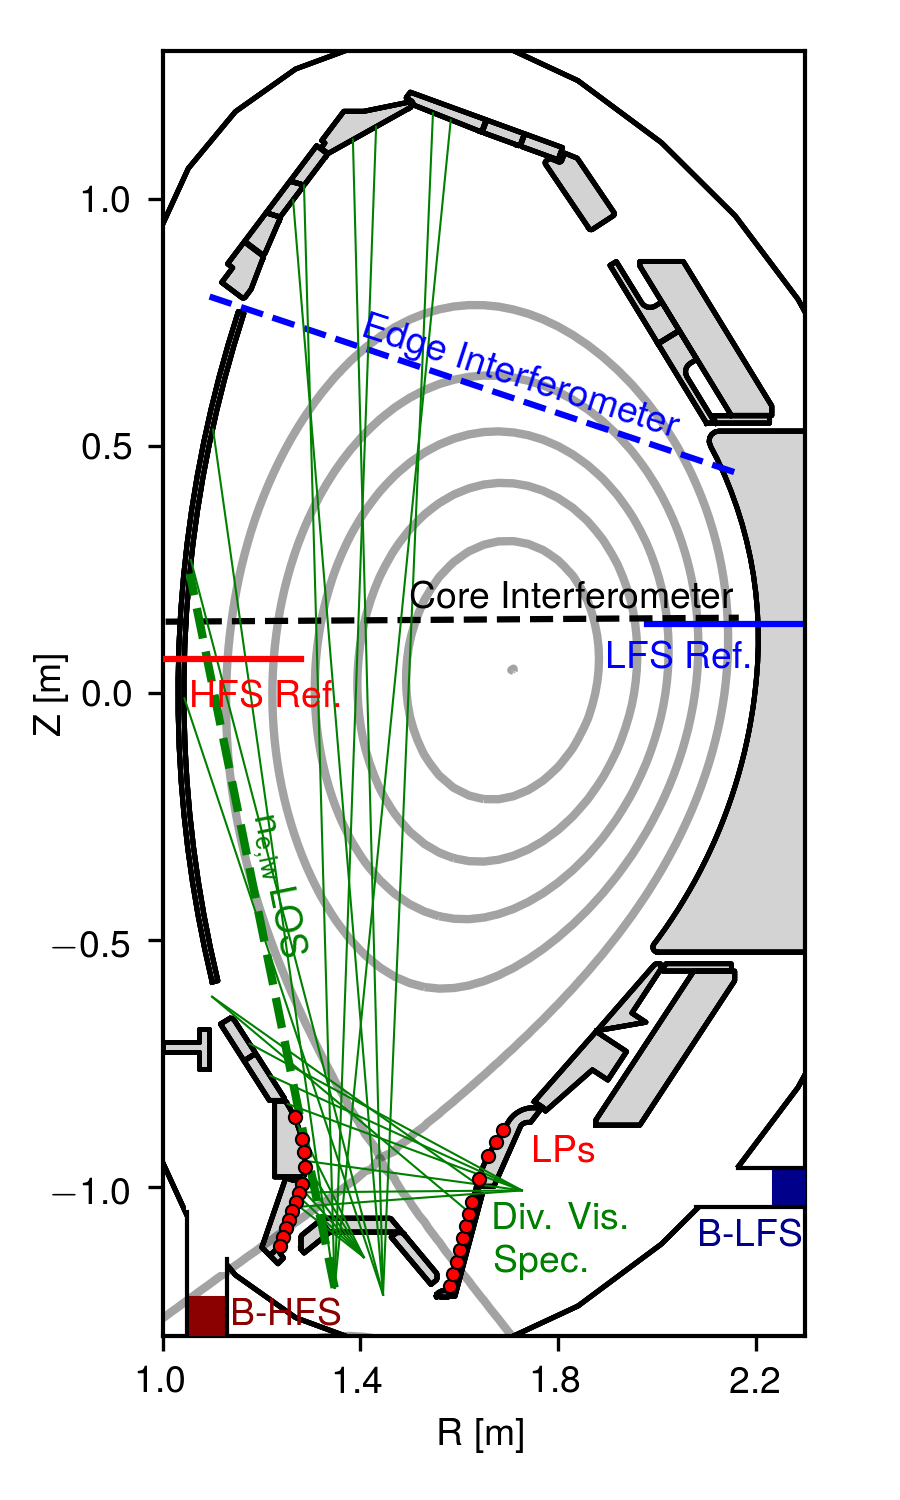
\includegraphics[]{Figure1.png}
    \caption[Main diagnostics used.]{Poloidal location of diagnostics. Lines of sight of the LFS and HFS reflectometry (blue and red at the midplane, respectively); edge and core interferometers (dashed blue and black); divertor Langmuir probes (LPs); Lines of sight of divertor visible spectroscopy in green (special LOS grazing the inner divertor wall, $n_{e,iw}$ highlighted); the LFS and HFS baratrons, represented by B-HFS (dark red) and B-LFS (dark blue), respectively.}
    \label{fig:diag_distribution}
\end{figure}


The main diagnostic explored in this work is the LFS/HFS reflectometer\cite{Silva1996}, installed close to the magnetic midplane of AUG. It is an O-mode reflectometer, meaning its measurements are independent of magnetic field. %A comparison between the reflectometer other density profile diagnostics follow in section \ref{section:hfslfscomphmode}.
Flush mounted Langmuir probes (LPs)\cite{weinlich1996flush} are used to measure ion fluxes at the divertor targets (as well as density and temperature). Two baratrons are used to measure neutral pressure at both the inner and outer divertor. 

%%%%%%%%%%%%%%%%%%%%%%%%%%%%%%%%%%%%%%%%%%%%%%%%%%%%%%%%%%%%%%%%
\section{Overview of the divertor detachment evolution}
\label{section:overviewdivdetevol}

In the next generation of fusion devices, a reduction of the expected power loads on the plasma facing components is mandatory. Detached operation is a requirement, with high densities and low temperatures at the divertor targets achieved at high fuelling rates. The effect of plasma fuelling, additional heating, and seeding have been explored thoroughly on AUG (e.g \cite{kallenbach2018parameter,Potzel2015a,Bernert2013a}) with the goal of optimising the design of future reactors. Figure \ref{fig:evo_30554} presents the temporal evolution for an H-mode discharge where first the input power and the fuelling are increased and, later on, nitrogen seeding is injected. Also shown in figure \ref{fig:evo_30554} is the evolution of the density profiles in the divertor volume measured by Stark broadening in the inner target by the horizontal and vertical LOS and the particle flux, $\mathrm{\Gamma_{D^{+}}}$, profiles measured by Langmuir probes in the inner divertor.

ELMs lead to large variations in the divertor parameters making the interpretation of Stark broadening and Langmuir probe data difficult and partially masking the evolution of the inter-ELM parameters. To study the density evolution during the entire discharge measurements during ELMs have been removed and therefore the figure displays essentially the inter-ELM evolution. Later it will be shown that the detachment conditions vary strongly along the ELM cycle.

Three distinct discharge phases may be identified according to auxiliary heating power, fuelling, and seeding levels. In the first H-mode phase (up to $2.8\,s$, the area shaded in red) moderate NBI power and gas fuelling are applied. In this phase the inner divertor is partially detached ($\mathrm{\Gamma_{D^{+}}}$ decreases with line-averaged density, see figure \ref{fig:evo_30554}e) and a high density in the inner divertor volume is observed (far-SOL at the height of the X-point, see figure \ref{fig:evo_30554}c,d) indicating that the HFSHD is already present in the divertor region. In a second phase (from $3\,s$ to $3.5\,s$, the area shaded in green) both the NBI power and gas fuelling rate are increased. During this phase, the divertor HFSHD increases significantly, both in magnitude and in the spatial extent. Finally, at $3.5\,s$ (area shaded in blue), nitrogen is injected at a constant rate to cool the divertor leading to a clear enhancement in plasma confinement. During this phase, the HFSHD is mitigated and the particle flux to the inner target reduced indicating that complete detachment is approaching.

To follow the shot evolution at large time-scales, a set of selected densities from reflectometry profile data is chosen. From each individual profile, acquired every $1\,ms$, the temporal evolution of each density layer is tracked for inter-ELM periods only. The data can then be used for comparison with other $1D$ time-traces by analysis of the iso-density contours. To remove ELM signatures from the iso-density layers, a Kalman filter\cite{kalman1960new} is employed, which eases the interpretation of their temporal evolution. The filtering approach is similar to the one used in real time reflectometry applications\cite{Santos2012}. Figure \ref{fig:layers_nseed_30554} shows the evolution of the LFS and HFS iso-density lines (ELM removed) along the discharge with representative radial density profiles for the different phases shown in figure \ref{fig:perfs_30554}. The plasma confinement ($H_{98}$) increases during the seeded phase albeit fuelling and auxiliary heating remaining the same. The effect of nitrogen seeding on the edge density profiles and divertor conditions may be investigated comparing phases $II$ and $III$, as this is the main parameter changed between the two phases.

\begin{figure}[!bt]
    \centering
    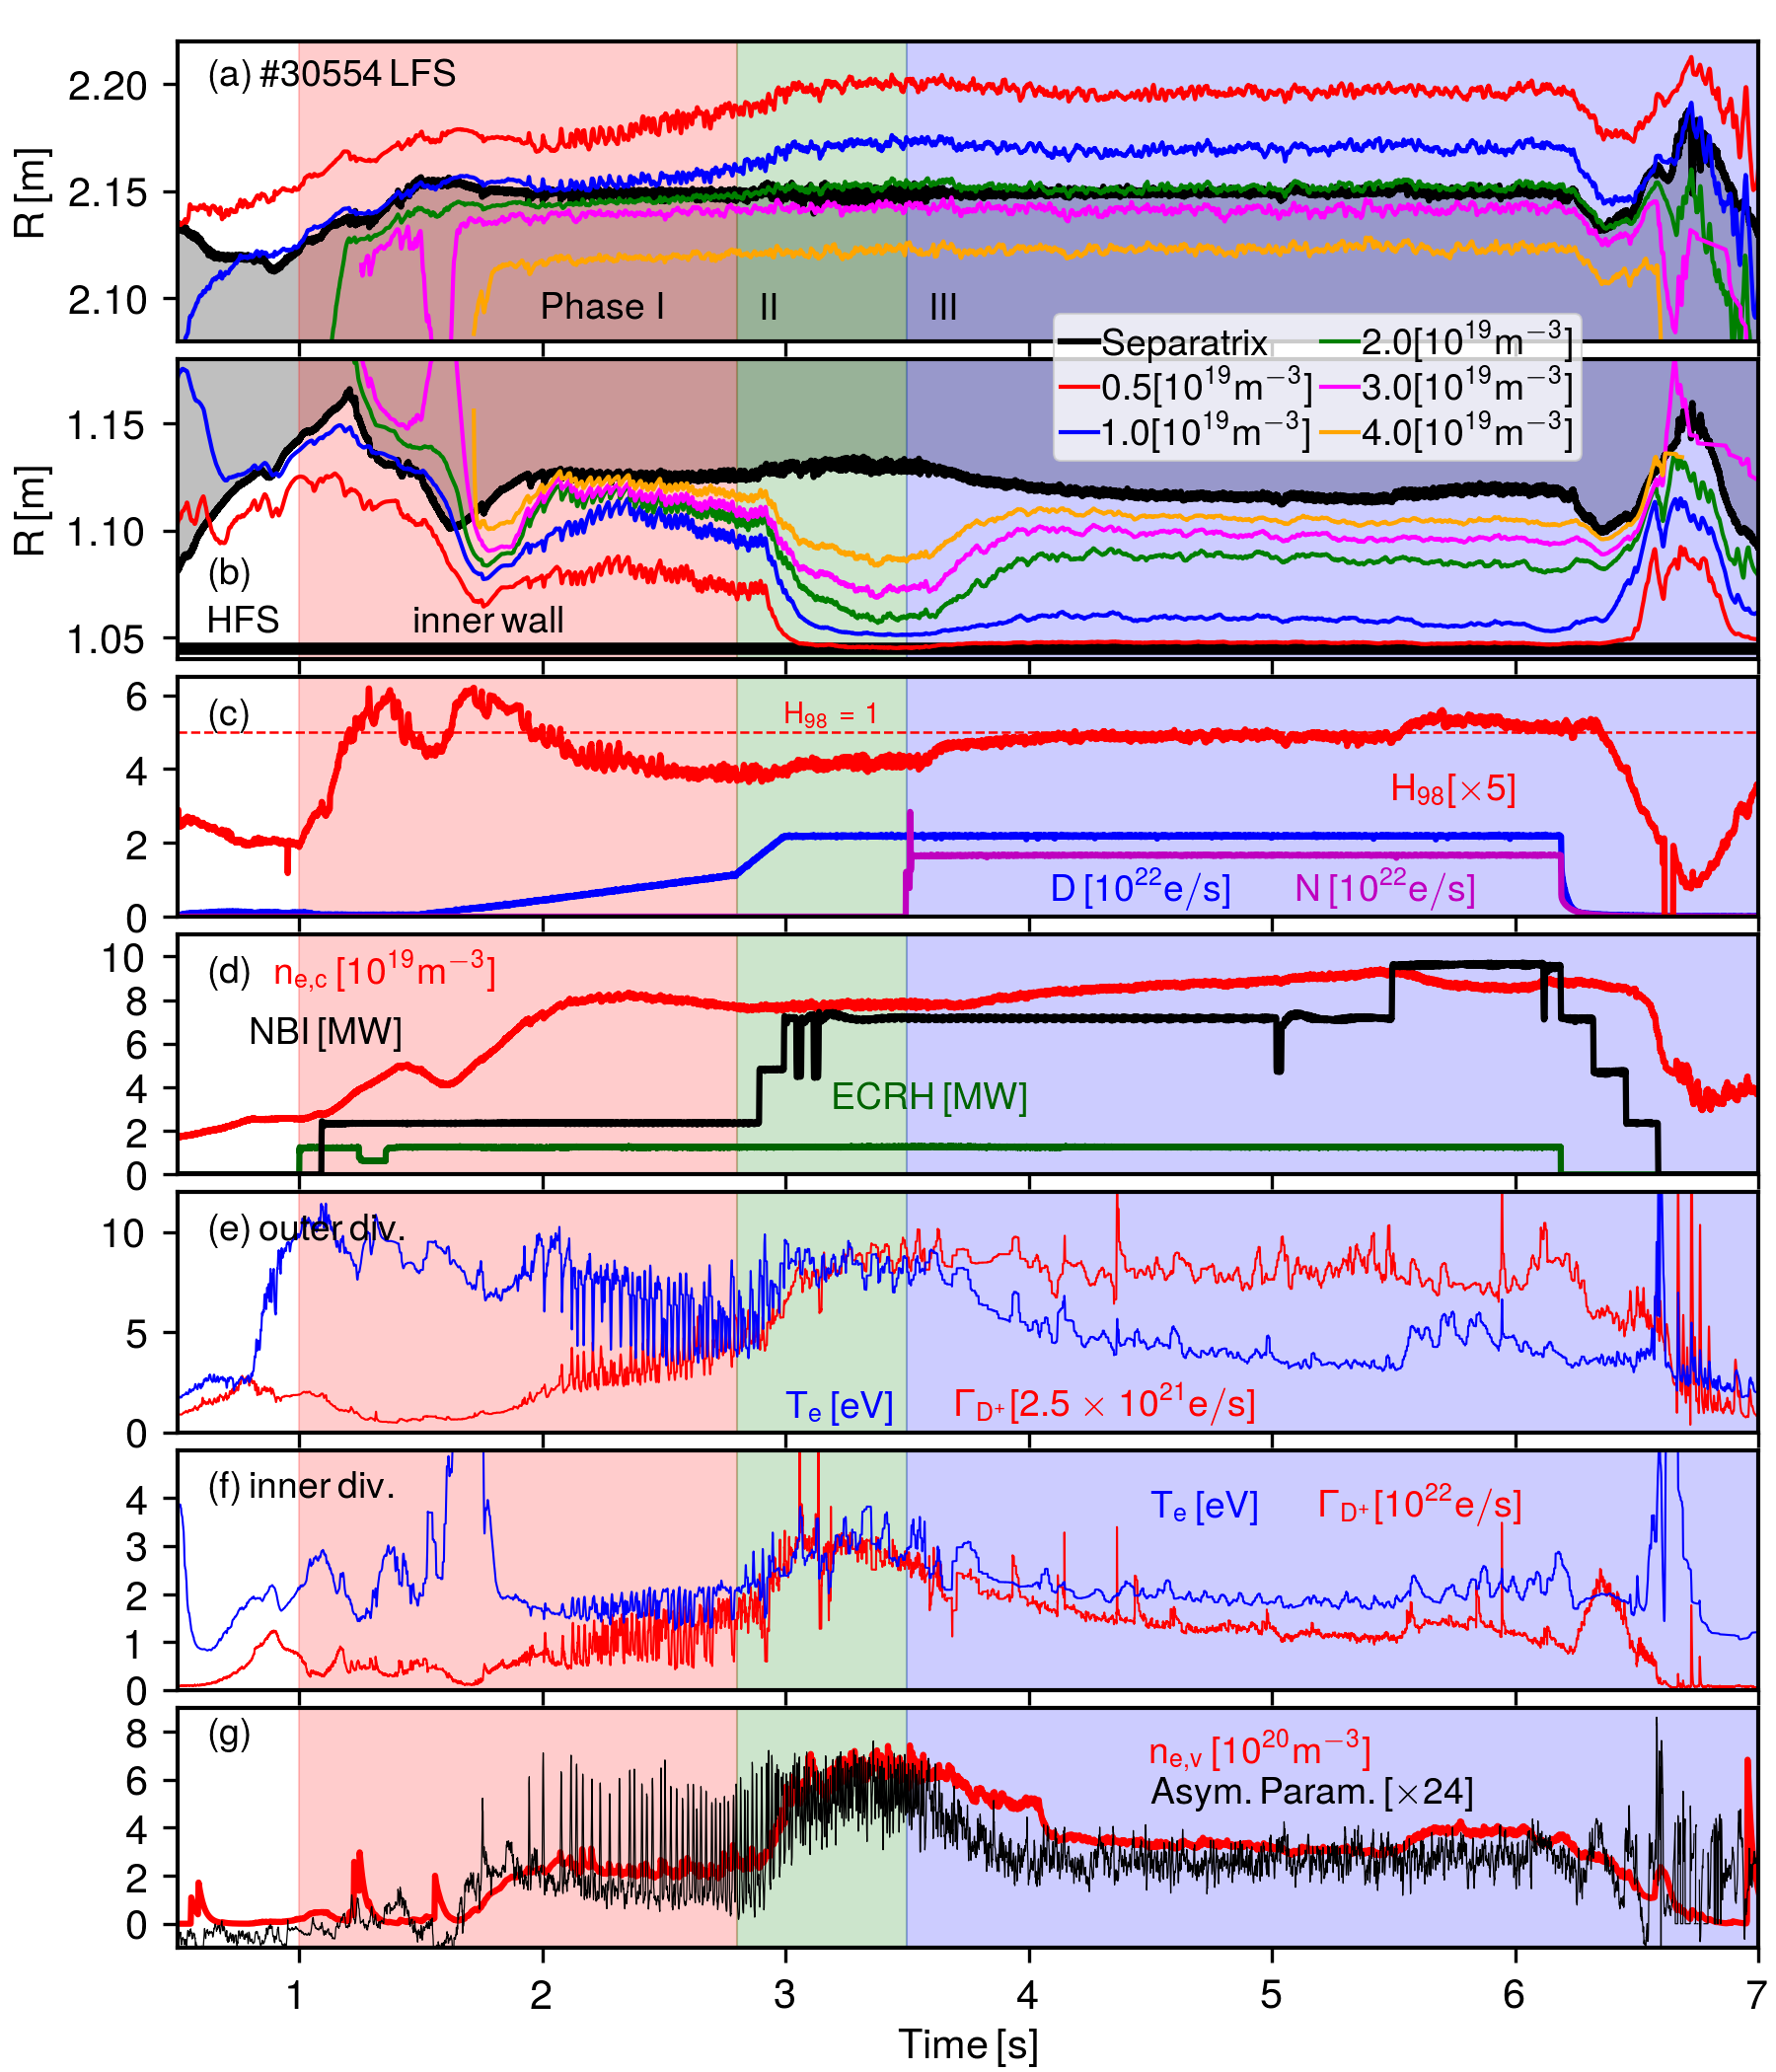
\includegraphics[]{Figure2.png}
    \caption[Overview of discharge \#30554.]{Trajectories of selected density layers at LFS (a) and HFS (b) for discharge \#30554 with nitrogen seeding from profile reflectometry; fuelling rate, nitrogen seeding rate and $H_{98}$ (c); central line-averaged density, NBI and ECRH heating power (d); $\mathrm{\Gamma_{D^{+}}}$ and $T_e$ measured by Langmuir probes near the outer (e) and inner divertor strike-point (f); asymmetry parameter and density in the divertor volume (g). Reflectometry and Langmuir probe signals during ELMs have been removed.}
    \label{fig:evo_30554}
\end{figure}

To understand the evolution of the midplane HFSHD, our attention is turned to the behaviour of the divertor parameters. Also shown in figure \ref{fig:layers_nseed_30554} are the particle flux and the electron temperature measured by the target Langmuir probes near the inner and outer strike-points to assess the evolution of divertor detachment along the discharge. As illustrated, $\Gamma_{D^{+}}$ increases at the inner divertor and even more noticeably at the outer target when the input power is stepped up suggesting a regression in the detachment state. When nitrogen seeding is injected both $\Gamma_{D^{+}}$ and $T_e$ decrease sharply particularly in the inner divertor (with $T_e$ values below $5\,eV$) indicating that full detachment is approached. The average density in the divertor volume measured by the Stark broadening diagnostic in the inner divertor is also shown in figure \ref{fig:layers_nseed_30554}.

During the phase $II$ of the discharge, the divertor HFSHD increases significantly in magnitude but then when nitrogen seeding is injected at a constant rate to cool the divertor, the divertor HFSHD is clearly mitigated. To infer the magnitude of the HFSHD, an asymmetry parameter (introduced in \cite{guimarais2017poloidal}) based solely on reflectometry data is calculated and compared to divertor visible spectroscopy. A very good agreement is observed between the evolution of the asymmetry parameter and that of the density in the divertor volume, $n_{e,v}$, confirming the strong influence of the divertor conditions on the midplane density profiles at HFS also in H-mode. Density profiles during ELMs were not removed when calculating the asymmetry parameter, revealing that this parameter exhibits strong variation during the large type-$I$ ELMs characteristic of the first discharge phase (described later in section \ref{section:hfslfselmcycle}). It is important to note that the asymmetry parameter cannot be calculated for most H-mode scenarios as the HFS profiles are often crashed against the HFS wall. Since in some cases no valid integration region is available, the asymmetry parameter remains undefined.

In spite of the roughly constant line-averaged density throughout the discharge, the behaviour of the HFSHD changes strongly. The increase of the heating power and fuelling rate leads to the development of the HFSHD that is then reduced when nitrogen is injected. Already in the first discharge phase, a clear LFS/HFS asymmetry in the density profile is observed favouring the HFS indicating the presence of a HFSHD as expected due to the moderate values of input power and fuelling. As illustrated in Figure \ref{fig:layers_nseed_30554}, an increase in the deuterium fuel rate leads to an outward shift of the LFS density profile and to a small increase in the HFS SOL density. In the second phase, both the fuelling and the input power are raised leading to a stronger HFSHD clearly identified by the quick movement of the density layers towards the inner wall. The SOL width at the LFS reaches a maximum during this period as a consequence of the high fuel rate (see figures \ref{fig:layers_nseed_30554} and \ref{fig:perfs_30554}), confirming the results shown in section \ref{sec:fuel_power}. Again most of the changes at the LFS are seen in the SOL (for densities below $2.0\times10^{19}m^{-3}$) with modest modifications in the pedestal region. At the HFS, the HFSHD causes the density profile to be pressed against the inner wall. 

\begin{figure}[!bt]
    \centering
    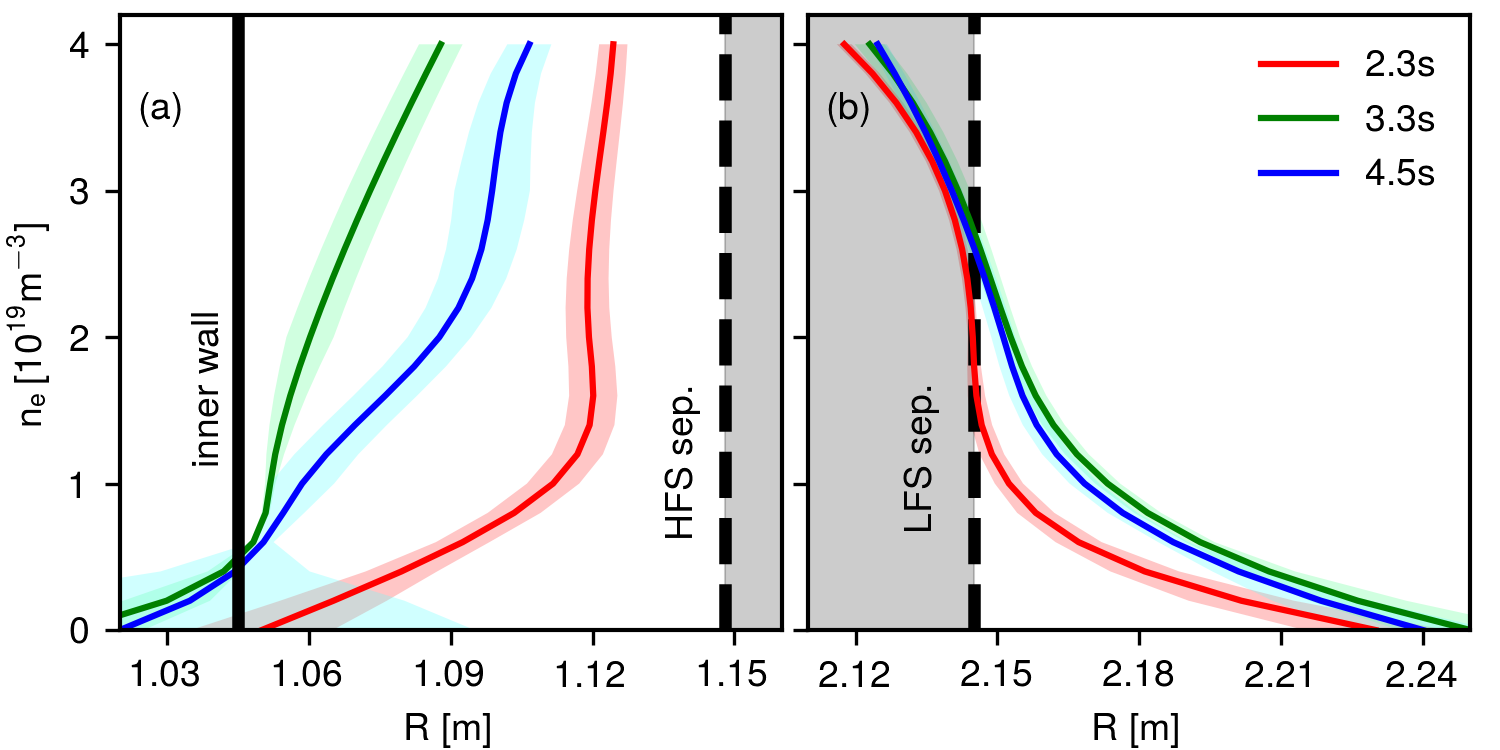
\includegraphics[]{Figure3.png}
    \caption[Density profile evolution for discharge \#30554.]{Evolution of the density profiles from reflectometry at (a) the HFS and (b) the LFS in normalised flux coordinates along the discharge \#30554 for the three discharge phases. Profiles are averaged over $20\,ms$.}
    \label{fig:perfs_30554}
\end{figure}

In phase $III$, nitrogen is injected that leads to a reduction of the HFSHD and also to a small reduction of the LFS SOL width. However, the density layers react slowly (over $\approx 0.5\,s$) to  the nitrogen injection.
%, around $0.5\,s$, period where some of the discharge parameters such as the line-averaged density and stored energy are also observed to vary. 
The addition of N seeding impacts on the LFS and HFS density profiles in a visibly different way. At the LFS, the SOL profiles seems to be slightly impacted and characterised by a marginal SOL narrowing (seen mainly in the trajectory of the $0.5\times10^{19}m^{-3}$ density layer in figure \ref{fig:layers_nseed_30554}), while on the HFS the effect on the average inter-ELM profile is significantly larger; nitrogen seeding strongly moves the density layers above $0.5\times10^{19}m^{-3}$ away from the inner wall as a consequence of a mitigation of the HFSHD. 

Similarly to the observation in L-mode, a clear correlation is observed between the evolution of the density in the divertor volume measured by spectroscopy and the asymmetry parameter estimated at the midplane (see figure \ref{fig:layers_nseed_30554}g). A HFSHD is observed to develop at the inner divertor during the first phase, that then increases strongly in magnitude when the input power and fuelling are stepped-up during the second phase reaching densities in the order of $60\times10^{19}m^{-3}$, in good agreement with the reflectometry data at the midplane. When nitrogen is injected in the third phase the density in the divertor volume decreases, again in agreement with observation at the midplane where the LFS/HFS asymmetry in density is reduced. Nitrogen actively mitigates the HFSHD, however, without completely suppressing it as the seeding rate cannot be increased further. The HFSHD is, therefore, an integral part of high-power H-mode operation in a tungsten wall machine like AUG.

%%%%%%%%%%%%%%%%%%%%%%%%%%%%%%%%%%%%%%%%%%%%%%%%%%%%%%%%%%%%%%%%
\section{The role of fuelling rate and input power}
\label{sec:fuel_power}

With the goal of disentangling the role of fuelling rate and input power on the midplane density profiles during inter-ELM periods, a discharge where these parameters are scanned independently is analysed. Three fuelling and three power steps take place independently in discharge \#30733, as shown in figure \ref{fig:layers_30733}. In order to produce a visible effect on the midplane density profiles, changes in the fuelling rate must be in the order of $\mathrm{10^{22}\,e/s}$. As the effect of the fuel rate and input power is different at the LFS and HFS, the two regions are analysed separately. At the LFS, the edge density is observed to respond clearly to the increase in the fuel rate leading to an outward shift of the profile, mainly seen in the density layers below $3.0\times10^{19}m^{-3}$ (see figures \ref{fig:layers_30733} and \ref{fig:perfs_30733}, comparing for instance profiles at $t=4.8\,s$ and $t=5.5\,s$). On the contrary, the input power has a minor impact of the density profiles as no changes are observed in the LFS SOL when the power is stepped-up (comparing for instance profiles at $t=3.8\,s$ and $t=4.8\,s$). In the confined region (shaded in grey), a modest reaction is observed to the variation in input power characterised by a small inward shift of the density layer that is then slowly recovered. Profiles shown in figure \ref{fig:perfs_30733} have been averaged over 20 ms, corresponding in general to about 10 profiles, as profiles measured during ELMs are discarded. To compensate for sporadic signal loss, a cubic spline has also been applied to the averaged profiles, to remove non-monotonicity. For low frequency type-I ELMs (about $50\,Hz$), this typically corresponds to one inter-ELM period while for high frequency ELMs (in the order of $200\,kHz$) will include several inter-ELM periods. Radial profiles in normalised flux coordinates for the time instants indicated are presented in figure \ref{fig:perfs_30733}. The line-averaged density exhibits a modest increase in spite of the large variation in the fuelling, as often is the case in ELMy H-mode discharges. As illustrated, $\Gamma_{D^{+}}$ at the outer target increases with fuelling showing that this divertor region is still attached. $T_e$ does not show significant changes throughout the discharge except a reduction at the inner target when the input power is stepped-up probably associated with an increase in the HFSHD.

\begin{figure}[!hbt]
    \centering
    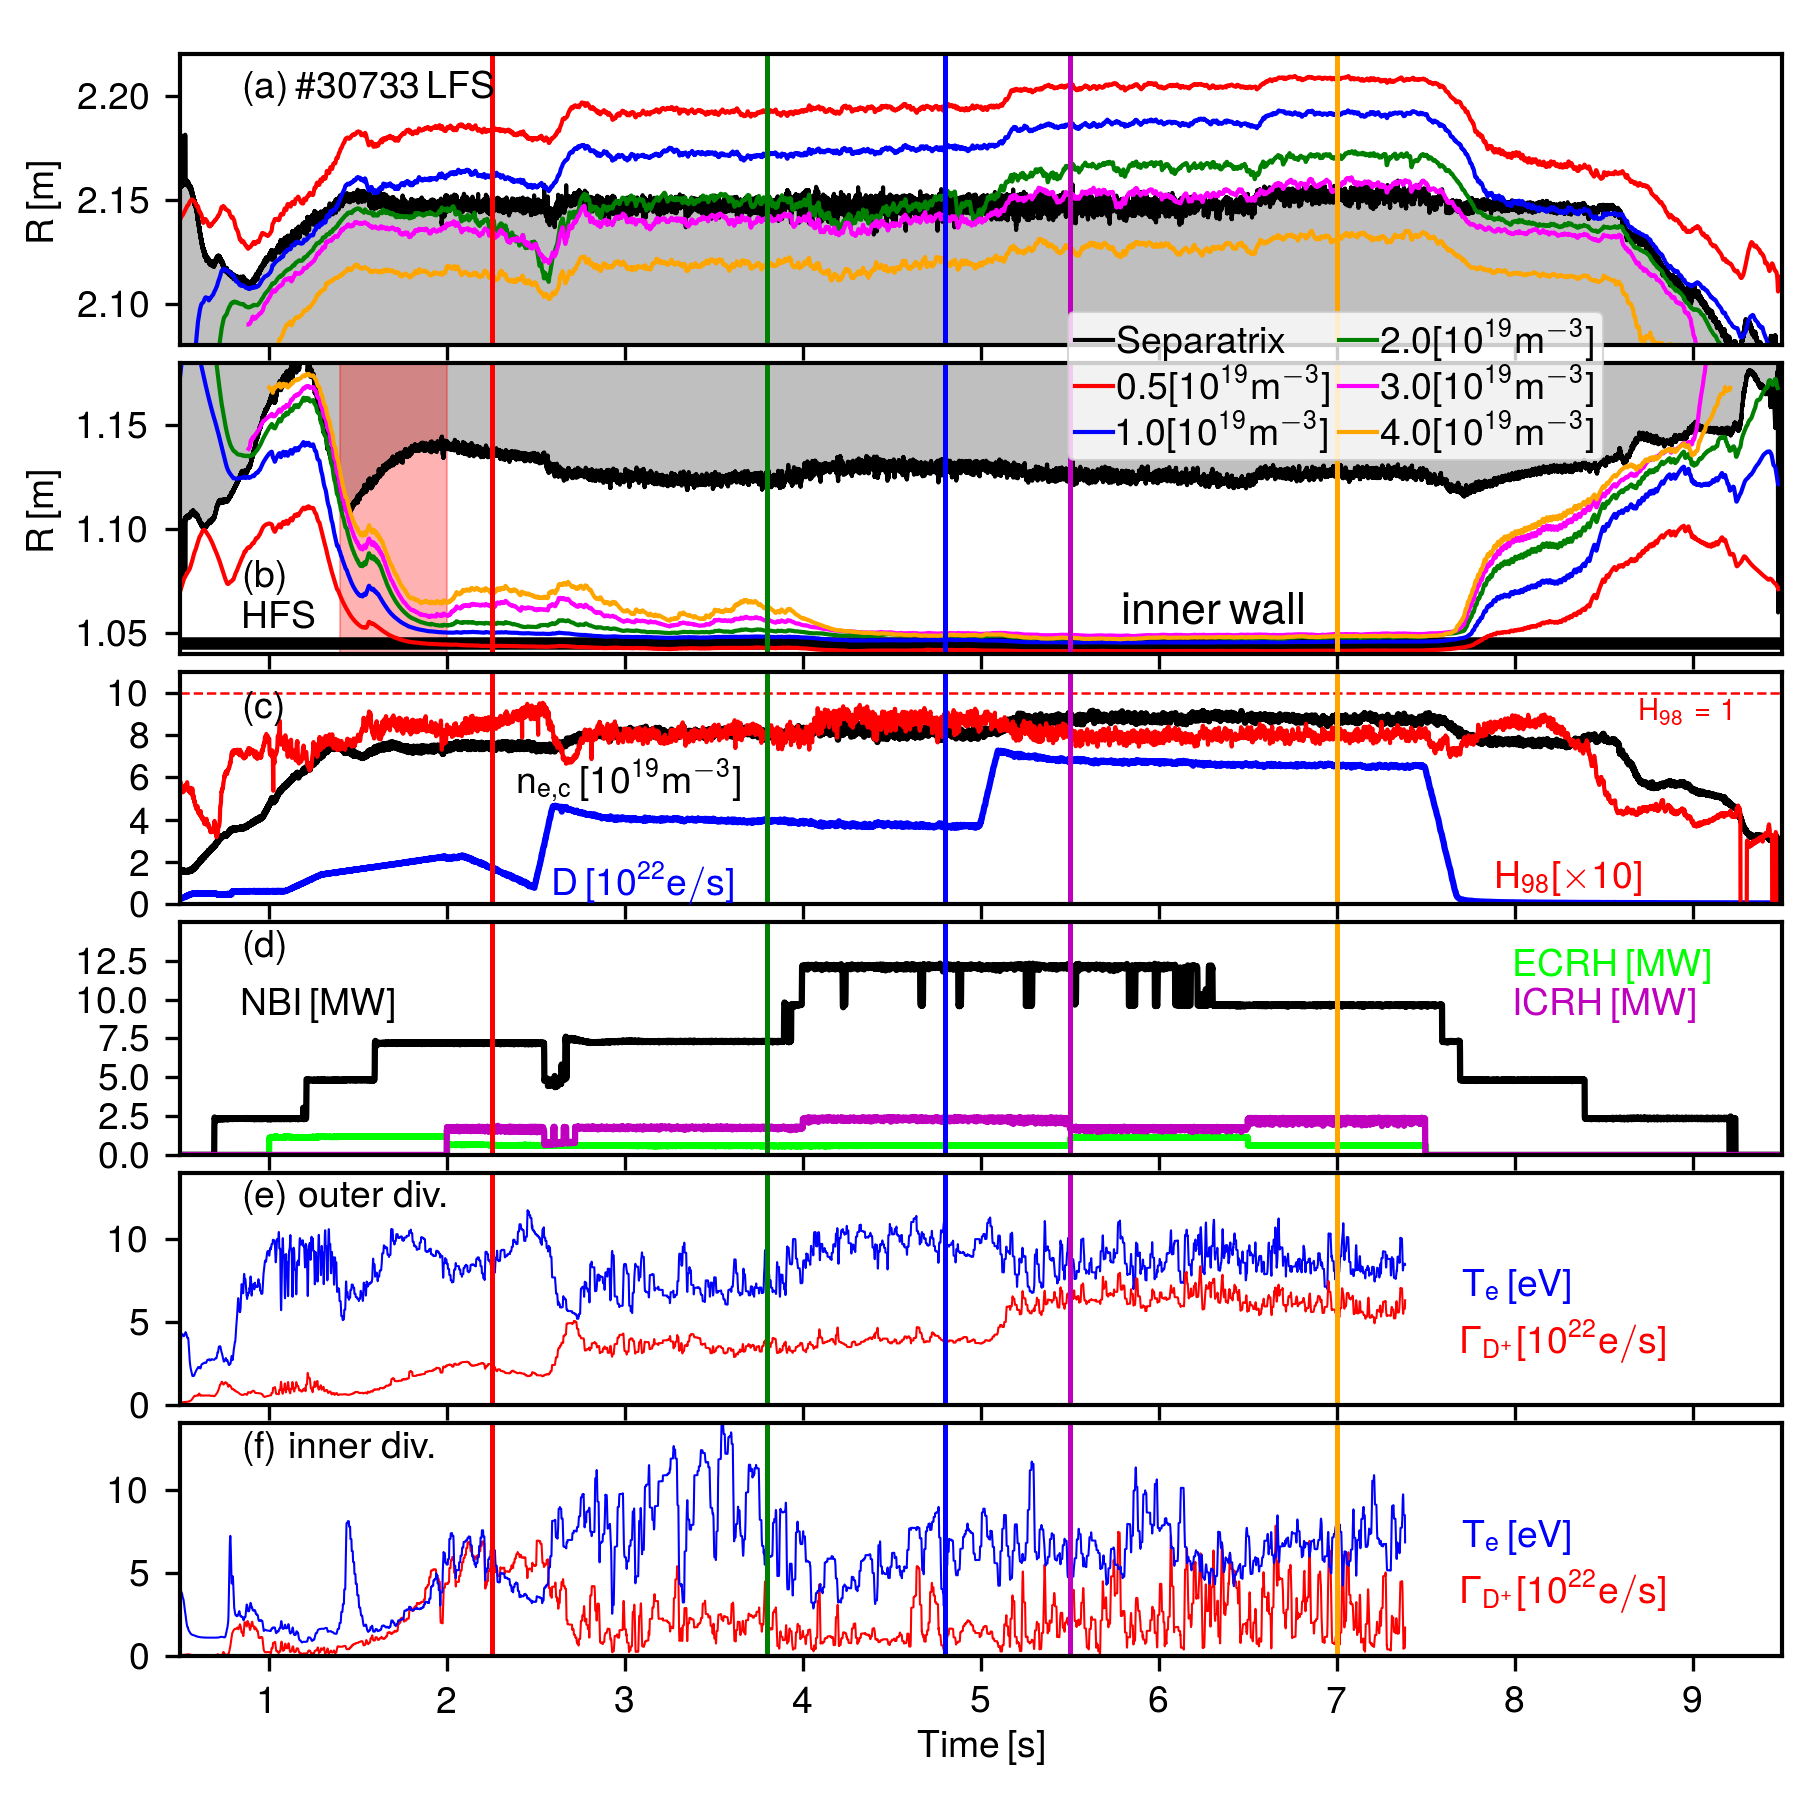
\includegraphics[]{Figure4.png}
    \caption[Overview of discharge \#30733.]{Trajectories of selected density layers at LFS (a) and HFS (b) for discharge \#30773 from profile reflectometry; fuelling rate, central line-averaged density and $H_{98}$ (c); NBI and ECRH heating power (d); $\mathrm{\Gamma_{D^{+}}}$ and $T_e$ measured by Langmuir probes near the outer (e) and inner divertor strike-point (f). Reflectometry and Langmuir probe signals during ELMs have been removed.}
    \label{fig:layers_30733}
\end{figure}

\begin{figure}[!bt]
    \centering
    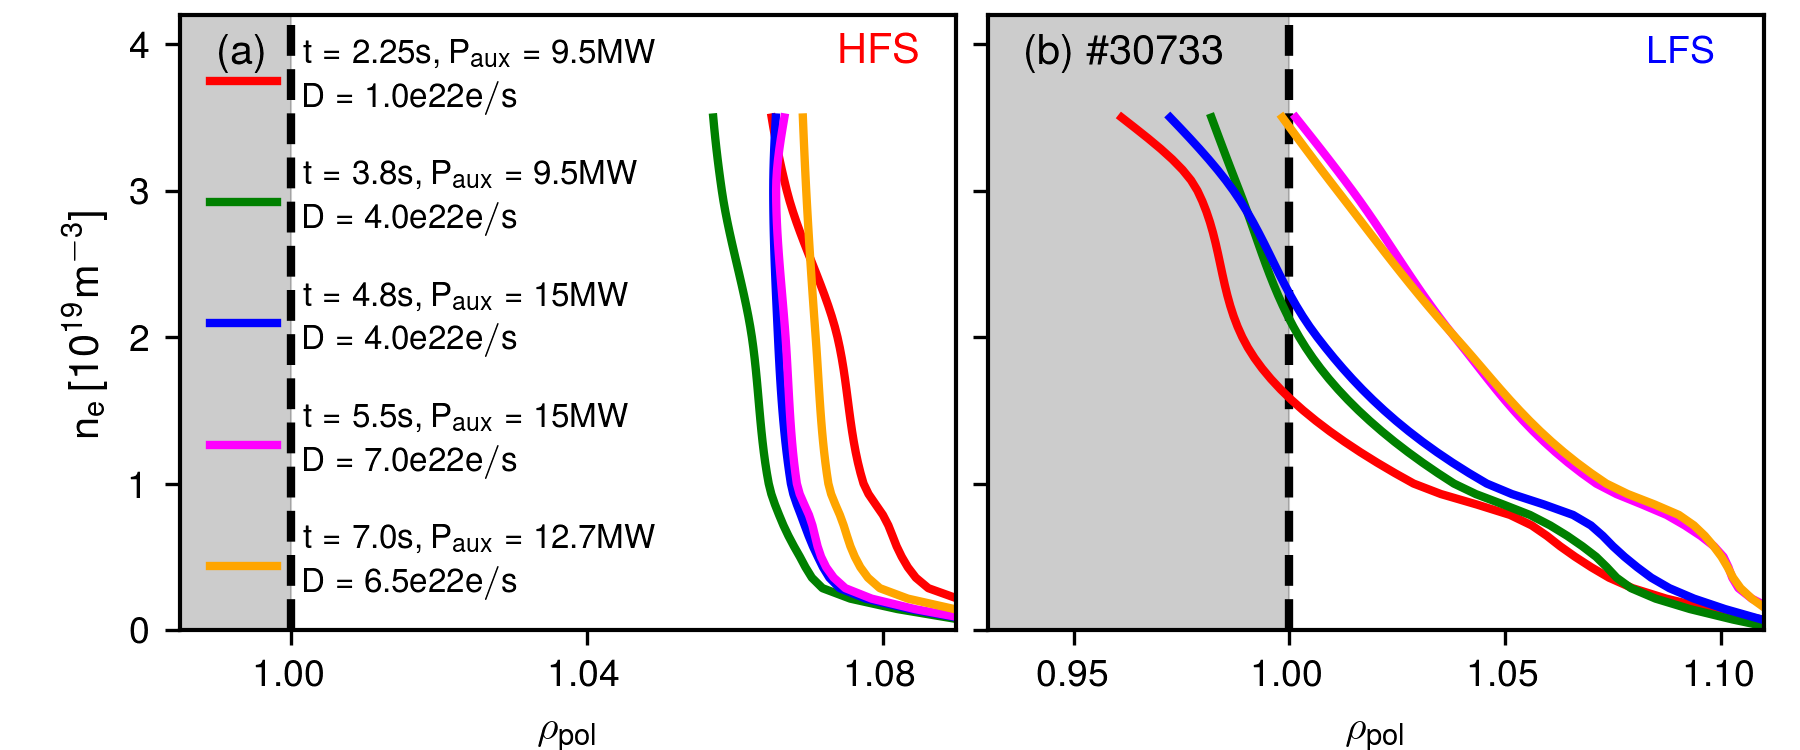
\includegraphics[]{Figure5.png}
    \caption[Density profile evolution for discharge \#30733.]{Evolution of the density profiles from reflectometry at (a) the HFS and (b) the LFS in normalised flux coordinates along the discharge \#30733 for the time instants indicated in figure \ref{fig:layers_30733}. Profiles are averaged over $20\,ms$.}
    \label{fig:perfs_30733}
\end{figure}

The increase of the fuelling rate is often associated with a degradation of plasma confinement. However, no marked changes occur when the HFSHD is rapidly formed suggesting that confinement properties are not directly associated with modifications in the HFSHD, as observed in L-mode\cite{guimarais2017poloidal}. Also shown in figure \ref{fig:layers_30733} is the particle flux and the electron temperature measured by a divertor target Langmuir probe near the inner and outer strike-points to assess the evolution of divertor detachment along the discharge. As illustrated, both $\Gamma_{D^{+}}$ and $T_e$ decrease with fuelling at the inner divertor ($T_e$ reaching values below $5\,eV$) indicating partial detachment while at the outer target $\Gamma_{D^{+}}$ increases with fuelling showing that this divertor region is still attached. Note that the increase in the fuelling rate leads to faster ELMs. Above a certain ELM frequency measurements during ELMs are difficult to remove resulting in the apparent increase in the signal fluctuations. 

At the HFS, an HFSHD is observed to exist from  early in the discharge ($t > 1.5\,s$) as consequence of the relatively high input power and line-averaged density. The HFSHD gets stronger when the gas is raised at $t = 2.5\,s$ but augments even further when the input power is stepped up. As the density layers are already “saturated” (profiles crashed against the inner wall), no further evolution is detected. The effect of the input power is therefore clearly different at LFS and HFS: it increases strongly the HFSHD while the LFS profiles are not significantly modified.

Plasma confinement is also differently influenced by the variation in input power and fuelling (see figure \ref{fig:layers_30733}). Confinement is observed to improve slightly when the power is stepped up and to degrade when the fuel rate is increased, corresponding to a different dependence on the plasma parameters than that observed for the HFSHD, which increases with both input power and fuelling.

To better visualise the dependence of the LFS midplane density on fuelling and input power, the relative variation of the midplane density at different radial locations with fuelling rate is shown in figure \ref{fig:pres_fuel_30733} for two power levels ($P_{in}=9.2$ and $16.4\,MW$) for discharge \#30733. Densities at different locations were estimated for the times used in  figures \ref{fig:layers_30733} and \ref{fig:perfs_30733} considering as a reference for the density variation the profiles at $t=2.35\,s$. Data for the SOL and separatrix regions are from reflectometry while Thomson scattering data is used in the confined region ($\rho=0.90$). As shown before, the SOL and separatrix density increase with fuelling particularly at the highest fuelling rate (SOL density duplicates when the fuelling rate is varied by a factor of two), while the density in the confined region does not change significantly. An increase in the input power (comparison between star and circle symbols at a fuelling rate of $\approx 4\times10^{22}\,e/s$) does not modify the LFS density in the confined region and leads to a modest density increase ($<20\%$) in the SOL and at the separatrix. 

\begin{figure}[!bt]
    \centering
    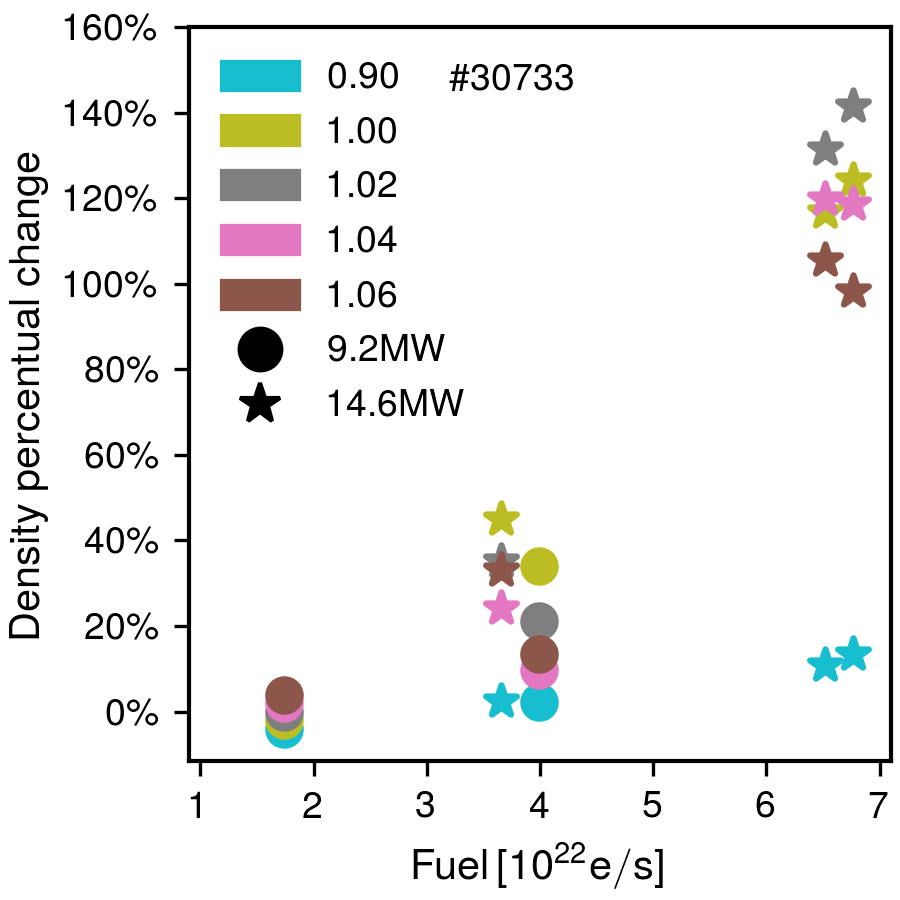
\includegraphics[]{Figure6.png}
    \caption[Relative variation of the LFS midplane density for \#30733.]{Relative variation of the LFS midplane density at different radial locations with fuelling for $P_{in}=9.2$ and $16.4\,MW$ for discharge \#30733. Data for the SOL and separatrix regions are from reflectometry while Thomson scattering data is used at $\rho=0.90$  (averaged over $50\,ms$).}
    \label{fig:pres_fuel_30733}
\end{figure}

\begin{figure}[!bt]
\centering
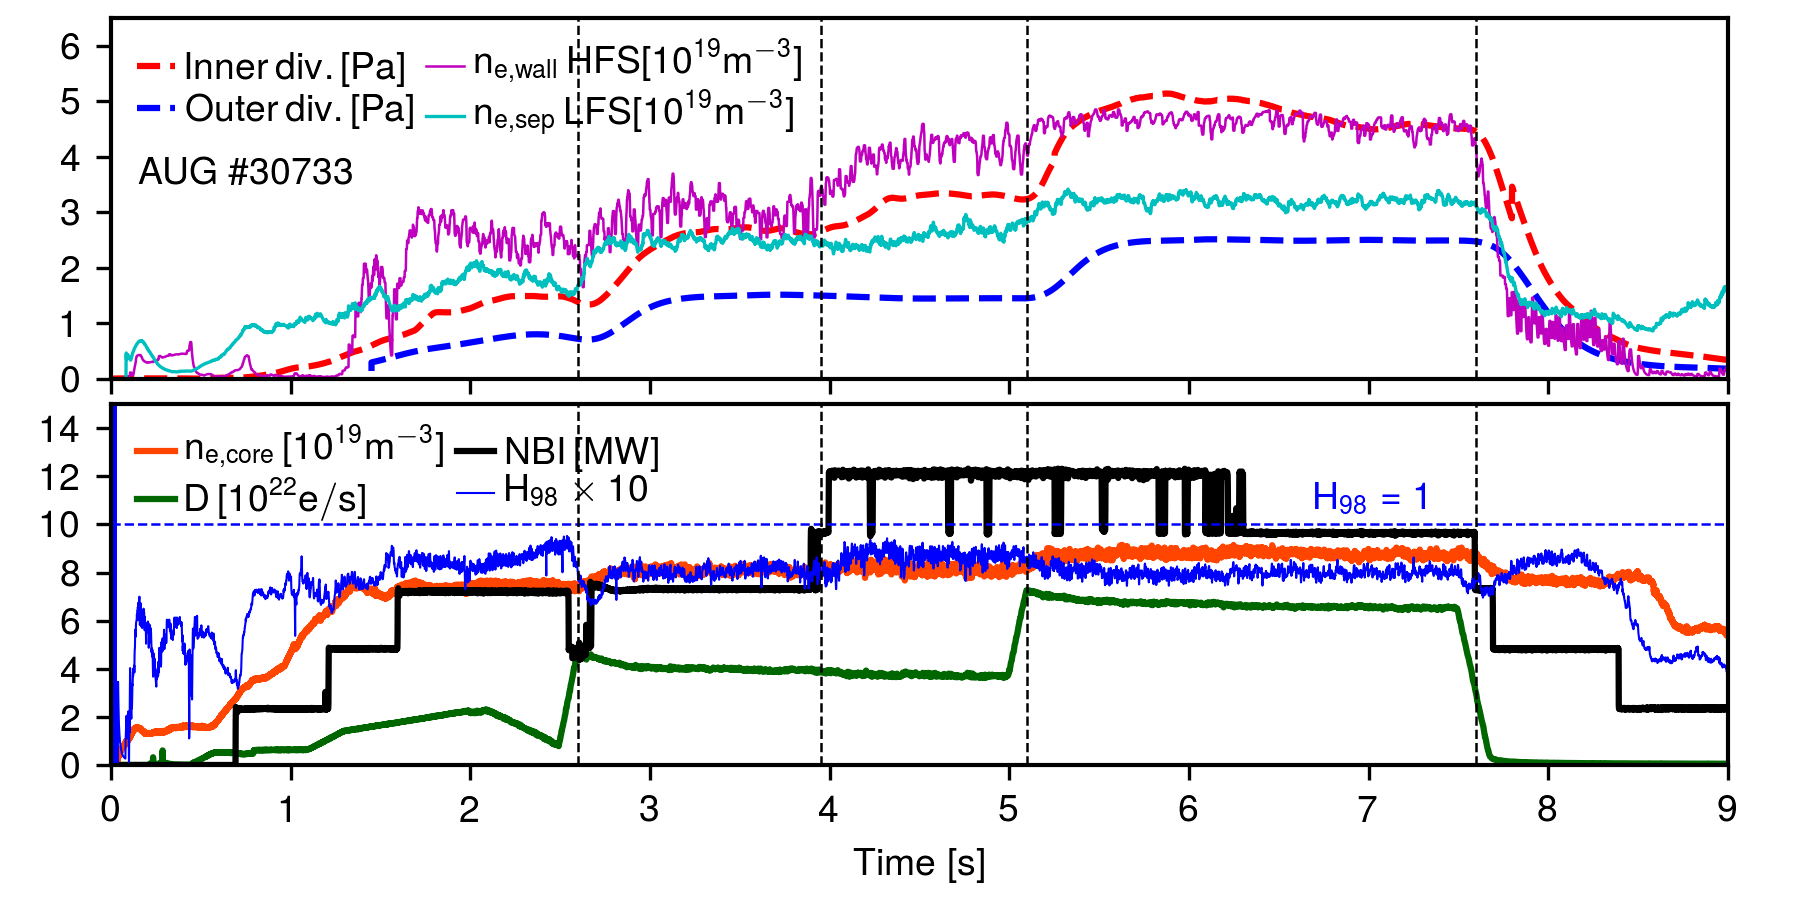
\includegraphics[]{Figure7.png}
\caption[Baratron neutral pressure evolution for \#30733.]{Top: Evolution of the neutral pressure measured by the baratrons at the inner (blue) and outer (red) divertor together with that of the LFS separatrix density estimated from reflectometry (cyan) and estimated maximum density measured by reflectometry at the inner vessel wall (magenta). Bottom: core line-averaged density (red), deuterium fuelling rate (green), NBI heating power (black) and $H_{98}$ factor (blue) for discharge \#30733.}
\label{fig:baratron_30733}
\end{figure}

The link between the HFSHD, divertor conditions and midplane density profiles, can be further explored by analysing the neutral pressure data measured by baratrons below the inner and outer divertor. Kallenbach has shown recently\cite{kallenbach2018parameter} that the upstream separatrix density for H-mode plasmas is strongly correlated with the outer divertor neutral pressure. Figure \ref{fig:baratron_30733} displays the evolution of the neutral pressure in the inner and outer divertor again for discharge \#30733, measured by the baratrons, together with the estimated separatrix density at the LFS from reflectometry. As the deuterium fuelling is raised both the outer divertor neutral pressure and the midplane SOL LFS density increase confirming previous observations. On the contrary, when the input power is raised neither the divertor neutral pressure in the outer target nor the midplane SOL LFS density are significantly modified. These observations confirm the good correlation between the outer divertor neutral pressure and the SOL density at the LFS midplane. The upstream separatrix density (measured with Thomson scattering) for nitrogen seeded and unseeded H-modes depends on the divertor neutral pressure as: $n_{e,sep}^u \propto p_{0,div}^{0.3}$ 
\cite{kallenbach2018parameter}. Based on the separatrix density evolution measured by reflectometry for discharge \#30733 a stronger dependence is found: $n_{e,sep}^u \propto p_{0,div}^{0.47}$ as shown in figure \ref{fig:nsep_pzero}. The relation between the outer divertor pressure and the midplane density presented here is mainly for illustrative proposes; to obtain more accurate dependencies further studies are required with a more extensive data set.

\begin{figure}[!bt]
\centering
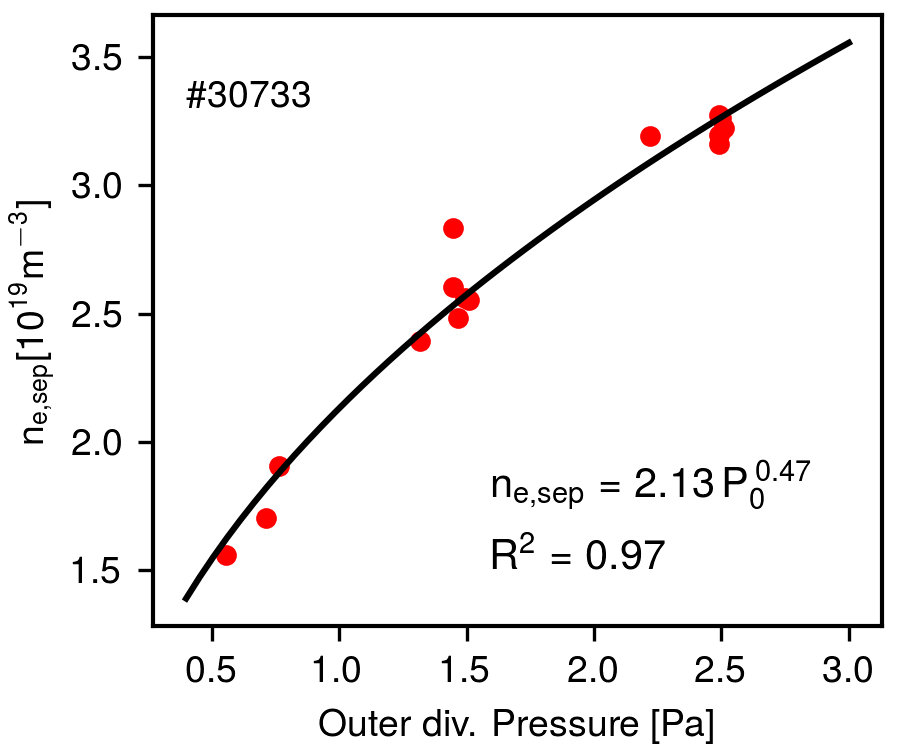
\includegraphics[]{Figure8.png}
\caption[Dependence of the LFS separatrix density on the outer divertor pressure for discharge \#30733.]{Dependence of the LFS separatrix density measured by reflectometry on the outer divertor pressure for discharge \#30733. Separatrix location for reflectometry data given by CLISTE equilibrium\cite{mccarthy1999cliste}.}
\label{fig:nsep_pzero}
\end{figure}

Concerning the inner divertor, when deuterium fuelling is raised both the inner divertor neutral pressure and the  SOL density at the HFS midplane increase, similarly to the observation at the LFS. However, when the input power is raised both the inner divertor neutral pressure and the SOL density at the HFS midplane increase contrary to the observed at the LFS. The evolution of the inner divertor neutral pressure is consistent with that of the HFSHD as both are observed to increase with fuelling and input power.

Neutral pressure data gives further evidence that the LFS density profile is mainly influenced by the outer divertor target. An increase in the input power leads to a strong increase of the neutral pressure at the inner target and to a strengthening of the HFSHD but has a modest influence at the LFS (both at the midplane and outer divertor).    

%%%%%%%%%%%%%%%%%%%%%%%%%%%%%%%%%%%%%%%%%%%%%%%%%%%%%%%%%%%%%%%%Integrate at the divertor evolution part
\section{The effect of seeding}
\label{section:effectofseedinghmode}

A possible approach to solving the problem of the high heat loads in the divertor target is the distribution of the power over larger areas of the vessel wall by increasing the radiation. Neutral atoms and impurity ions that are not fully stripped of their electrons are excited in the plasma and emit line radiation leading to volumetric power loss in discharges with extrinsic impurity seeding. Low-Z and medium-Z species like nitrogen and neon are typically used. This increased power loss in the SOL and divertor is also used to promote detachment permitting the achievement of completely detached H-mode discharges in a full metal wall. Seeding is particularly important to achieve complete detachment at the outer target as scenarios with a detached inner divertor and an attached outer divertor are common on AUG. The selection of a divertor radiator requires impurities that radiate efficiently at the low electron temperatures characteristic for the divertor and SOL regions and not in the core of the plasma. Consequently, nitrogen appears as the main candidate, as detailed in \cite{kallenbach2013impurity}. Non-coronal enhancement of the radiative loss function can occur in fusion plasmas for instance due to plasma parameter variations caused by ELMs as indicated in recent studies \cite{Kallenbach2015}. 

%%%%%%%%%%%%%%%%%%%%%%%%%%%%%%%%%%%%%%%%%%%%%%%%%%%%%%%%%%%%%%%% Discard?
\section{Impact of HFSHD on the midplane density profiles and confinement}
\label{section:hfshdmidplanedenperfconf}

The structure of the pedestal density seems to play an important role in the pedestal stability and hence in the confinement, as recently observed in JET and AUG \cite{stefanikova2016effect,Dunne2017}. 
However, the physics mechanisms responsible for the changes in confinement with fuelling and seeding are not fully identified yet. A possible mechanics relating divertor and midplane conditions is the HFSHD as it extends from the divertor region up to the midplane with its magnitude depending on fuelling rate, input power, and seeding.
The divertor HFSHD was suggested to impact on the H-mode pedestal structure and stability leading to an outward shift of the density profile that causes a degradation of the pedestal top pressure and global confinement \cite{Dunne2017}.
The HFSHD is found to increase with heating power as the extra power across the separatrix leads to an increase of SOL ionisation sources in the inner divertor. On the contrary, the HFSHD decreases with seeding because the power reaching the inner divertor is reduced by radiation in the SOL. The HFSHD is, therefore, a plausible mechanism influencing the  confinement properties with nitrogen seeding that was first suggested by Potzel et al\cite{Potzel2015}. A good correlation was observed on AUG between the HFSHD formation and the evolution of the main plasma parameters such as $H_{98}$ or stored energy with respect to changes in seeding \cite{Potzel2015,Dunne2017}.  

Our results confirm that seeding leads to a reduction of the HFSHD, to an inward shift of the of the density profile and to a confinement enhancement in agreement with previous observations establishing a correlation between the reduction of the HFSHD and confinement improvement due to impurity seeding \cite{Potzel2015,Dunne2017}. This picture is further corroborated by the fact that an increase in the fuel rate leads to an increase in the magnitude of the HFSHD associated with a degradation in confinement. However, this degradation in confinement with fuelling is modest while the increase of the HFSHD is pronounced. In addition, the reduction of the separatrix density with seeding is much smaller than that with fuelling while the effect on confinement is more pronounced for seeding than for fuelling. This suggests that more is at play with respect to the effect of the HFSHD in confinement. This is further confirmed by the effect of the heating power that does not support the suggested detrimental effect on the HFSHD on confinement. An increase in the heating power leads to a strong increase in the HFSHD but also causes an enhancement in confinement (although modest). Furthermore, the HFSHD was observed to respond strongly to the heating power contrary to plasma confinement. The HFSHD is suddenly formed above a certain heating power or fuelling rate threshold without any simultaneous pronounced change observed in confinement. 

Fuelling and seeding have been observed to change significantly the divertor conditions, not only at the inner target where the HFSHD is observed but also at the outer one. In addition, the neutral pressure also changes significantly with the plasma parameters.
Kallenbach has shown that the upstream separatrix density presents a strong correlation with the divertor neutral pressure for nitrogen seeded and unseeded H-modes \cite{kallenbach2018parameter}.
Due to particle balance, the divertor pressure can be regarded as an engineering parameter largely proportional to the gas puff rate \cite{kallenbach2018parameter}. As shown in figure \ref{fig:baratron_30733} the pressure in the divertor gauges was found to respond strongly to the fuel rate both in the inner and outer target while responding to the input power only at the inner divertor. The density profile at the LFS is therefore observed to respond to changes in the outer target pressure while at the HFS is mainly influenced by the pressure at the inner target that is strongly influenced by the local divertor conditions. An increase in the power to the SOL leads to an enhancement of the HFSHD and to an increase in the neutral pressure at the inner target but has a weak effect on the outer target and LFS midplane.  The connection between the HFSHD and the LFS midplane profiles is therefore not always straightforward with respect to variations in the input power, contributing to the clarifications of the different behavior at the HFS and LFS midplane density.  
There is a correlation between the magnitude of the HFSHD and plasma confinement with respect to changes in impurity seeding but not with respect to the heating power suggesting the effect on the HFSHD on confinement has to be carefully validated. Our results indicate that the separatrix density at the LFS is better correlated with the neutral pressure at the outer target while the HFS SOL density (the HFS separatrix density cannot be measured) follows the neutral pressure at the inner divertor.   

Evidence for the existence of an HFSHD was found on ASDEX with a carbon wall, taking advantage of the information provided by a vertical $CO_2$ interferometer channel, localised at the HFS, that registered densities in excess of those expected from core/SOL parameters \cite{mccormick2009main}. A density threshold to the formation of the density front was found, corresponding to a Greenwald density fraction of 0.45. Midplane density profiles measured over more than one decade by reflectometry on AUG with a carbon wall were generally found to be HFS/LFS symmetric suggesting that the presence of a divertor density front occurs more frequently in full tungsten devices. In H-mode, evidence for the existence of a midplane HFSHD based on reflectometry on AUG with C wall was only found above a Greenwald fraction of about 0.7 while with W walls, it is observed above $f_{GW} \approx 0.55$. Carbon radiates mainly in the SOL (similarly to N) and is always present in the SOL as it was produced in carbon devices even at low temperatures. Therefore, the HFSHD is expected to be mitigated in C devices in a similar way that it is reduced with seeding in W devices.

Experiments in carbon wall devices have revealed the observation of an unstable dense, radiating region (MARFE), which becomes quickly unstable, most likely because of the self-amplifying effect due to the chemical sputtering that increases at low temperatures. For W based devices the cold detached divertor leads to lower sputtering and generally to a stable high radiation region.

%%%%%%%%%%%%%%%%%%%%%%%%%%%%%%%%%%%%%%%%%%%%%%%%%%%%%%%%%%%%%%%%
\section{HFS/LFS asymmetries along the ELM cycle}
\label{section:hfslfselmcycle}

In this section, the evolution of the midplane density profiles along the ELM cycle is investigated. A feature of H-modes are Edge Localized Modes (ELMs)\cite{zohm1996edge} that cause quasi-periodic relaxations of the pedestal gradients in the electron density and the electron and ion temperature, expelling energy and particles into the SOL and consequently leading to transient heat and particle loads onto the divertor targets. Fast measurements of the SOL parameters are crucial to the understanding of ELM dynamics and for the evaluation of the fluxes to the plasma-facing components.

In order to establish the effect of the different plasma parameters and divertor conditions on the midplane profiles, discharge \#30554 was again selected now with a focus in the ELM evolution. In the first H-mode phase moderate NBI power and gas fuelling are applied resulting in large amplitude low frequency ($50\,Hz$) ELMs. Figure \ref{fig:attached_elm_cycle} displays the evolution of the iso-density layers at the HFS and LFS for type-$I$ ELMs during the first phase of discharge \#30554 together with the particle flux, electron temperature, divertor shunt current and $D_\alpha$ emission at the inner and outer divertor target. During this phase the fuel rate and input power are moderate and inter-ELM midplane density profiles are roughly symmetric as shown previously. However, as illustrated in figure \ref{fig:attached_elm_cycle}, clear HFS/LFS asymmetries are observed during the ELM. Density layers at the LFS present the classical evolution corresponding to the ELM crash with SOL layers moving outwards and pedestal layers moving inwards. The observed time scales correspond to the typical ELM evolution on AUG with a collapse time in the order of $1\,ms$ and a recovery in the order of $2\,ms$, in agreement with data from the edge interferometer. Interestingly, the SOL density width seems to show a minimum around $2-3\,ms$ after the ELM crash, and then broadening slightly again later on before returning to their inter-ELM baseline position.

\begin{figure}[!bt]
\centering
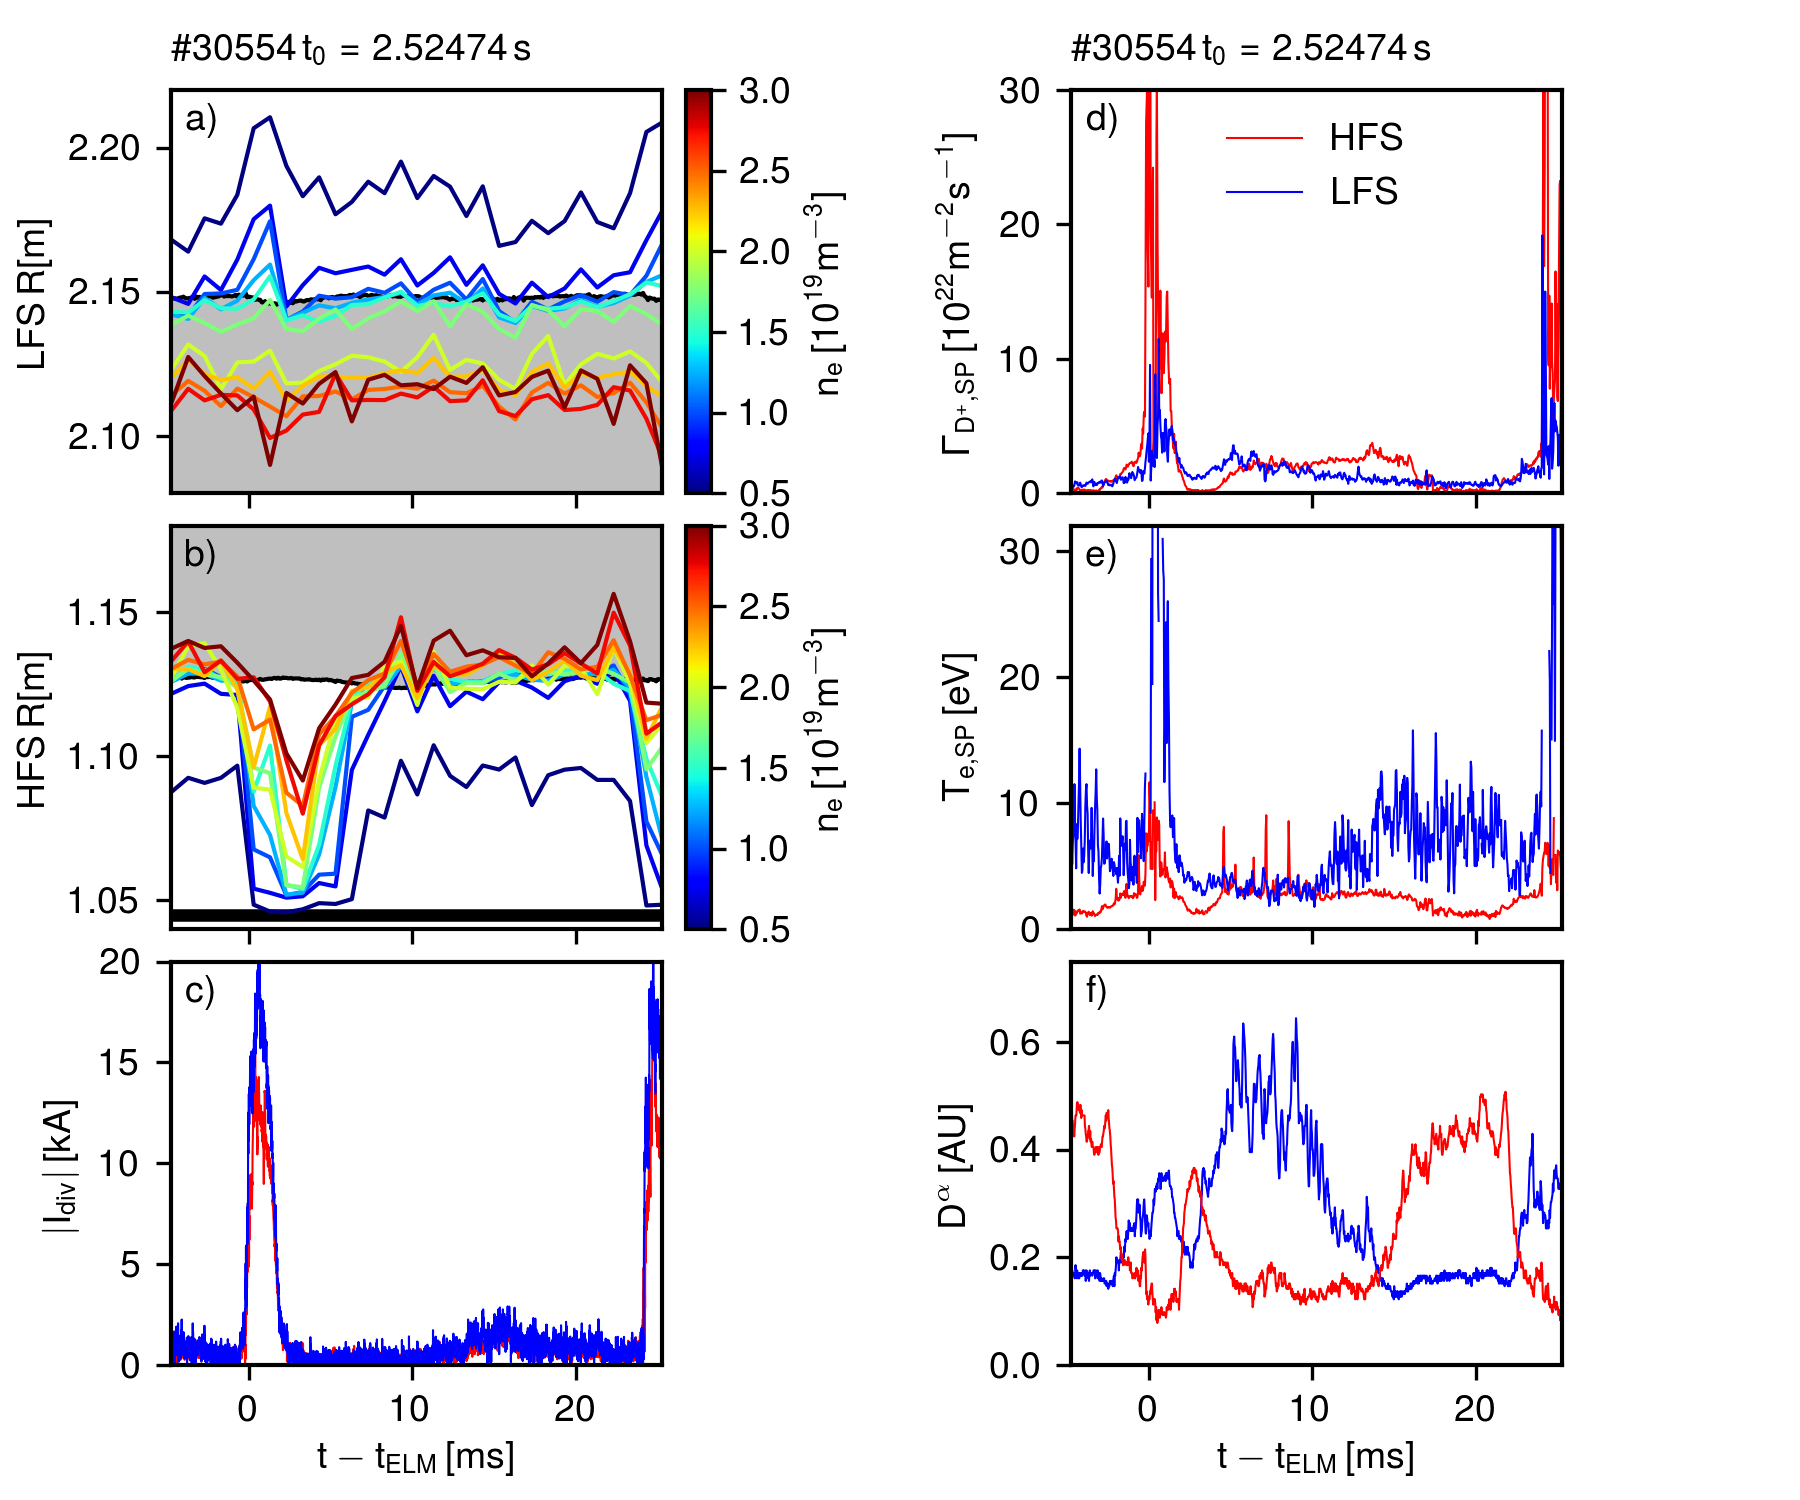
\includegraphics{fig119.png}
\caption{Evolution of the density layers from reflectometry at the LFS (a) and HFS (b) during type-$I$ ELM; together with the following parameters in the inner and outer divertor: divertor shunt current (c);  particle flux (d); electron temperature (e); and $D_\alpha $ radiation.}
\label{fig:attached_elm_cycle}
\end{figure}

The evolution of the HFS density layers is dramatically different. The ELM leads to a large increase in the SOL density characterised first by a fast evolution in a time scale below $1\,ms$ that is then followed by a slower outward movement of the layers with higher density up to $t-t_{ELM} \approx 2-3\,s$ ($t_{ELM}$ is defined as the beginning of the ELM crash). Afterwards, the profiles recover slowly reaching the inter-ELM profile only around $\mathrm{10\,ms}$ after the ELM crash. An HFS/LFS asymmetry is observed already during the pedestal collapse period with a larger SOL seen at the HFS, with the asymmetry getting stronger during the ELM recovery. The behaviour of the HFS midplane profile appears to be correlated with the detachment evolution at the divertor. The evolution in the divertor conditions is strongly influenced by the pedestal parameters during ELMs because transient changes in the heat and particle fluxes across the separatrix cause a strong modification in the SOL and divertor plasma.

A more detailed description of the evolution of the inner and outer divertor conditions along the ELM cycle can be obtained from the divertor Langmuir probes signals, also displayed in figure \ref{fig:attached_elm_cycle}. The large pre-ELM $D_\alpha$ emission at the inner target as well as the low $\Gamma_{D^{+}}$ and $T_e$ (that is below $5\,eV$) suggests that the inner divertor is at least partially detached before the ELM occurs. During the ELM crash the $D_\alpha$ radiation is reduced and the target $\Gamma_{D^{+}}$ and $T_e$ increase that can be interpreted as the inner divertor target becoming attached due to the particle and energy losses from the pedestal to the divertor. At about $t-t_{ELM} \approx 2\,ms$ the $D_\alpha$ radiation rises and the $\Gamma_{D^{+}}$ and $T_e$ are reduced again indicating a detachment of the inner target after the ELM. The degree of detachment is then reduced again around $t-t_{ELM} \approx 5\,ms$ as indicated by the increase in $\Gamma_{D^{+}}$ and $T_e$.

At the outer divertor target, the plasma is attached before the ELM with $\Gamma_{D^{+}}$ and $T_e$ increasing during the ELM crash. Then, starting around $t-t_{ELM} \approx 2\,ms$ and for a period of about $7-8\,ms$, the electron temperature is reduced to $\approx 5\,eV$ and $D_\alpha$ emission increases indicating that the outer divertor is partially detached.  After $\approx 10\,ms$, the outer target re-attaches again (increase in $T_e$ and decrease in $D_\alpha$) until the next ELM occurs.

In summary, just after the ELM crash, as the LFS density profiles recover, the outer divertor is in partial detachment and the inner divertor target is in full detachment. Interestingly, in the period from $\approx 4$ to $\approx 8$ ms the divertor parameters near the strike-point are roughly similar at the inner and outer divertor region suggesting a similar state of detachment. Afterwards, the detachment conditions have an opposite evolution at the inner and outer target, becoming more detached at the inner and more attached at the outer divertor. In a similar study of the detachment evolution along type-$I$ ELMs on JET \cite{field2017}, a momentary detachment after the ELMs was also found that was attributed to  both cooling of the SOL plasma by radiation from sputtered impurities and by a reduction of power losses crossing the separatrix after the ELMs, due to the lower pedestal pressure, which reduces the power to the divertor.

The period with a high degree of detachment at the inner divertor ($2 < t-t_{ELM} < 5\,ms$) corresponds to the phase were the midplane profiles are crashed against the inner wall suggesting the existence of a HFSHD during this period. Although the temporal resolution of the Stark broadening diagnostic does not permit following the evolution of the divertor HFSHD during the ELM cycle, the fact that the inner target is fully detached strongly suggests that a HFSHD is present at the inner divertor just after the ELM event. After $5\,ms$, the inner divertor moves to a partially detached state, recycling in the outer target is also reduced and a corresponding decrease of the midplane HFSHD is seen with the density profiles returning to pre-ELM values.

To overcome the limitation resulting from the modest temporal resolution of the reflectometry diagnostic, data from the different phases of discharge \#30554 has been conditionally averaged to obtain the typical evolution of the ELM for each phase using as reference the time of the ELM crash. Figure \ref{fig:elm_30554} displays the evolution of the iso-density layers at the HFS and LFS for average type-$I$ ELMs during the first phase of discharge \#30554 together with the particle flux to the inner and outer divertor target, also conditionally averaged. As expected the main features described above for the evolution along the ELM cycle is also seen in the conditionally averaged signals.

\begin{figure}[!hbt]
\centering
	\begin{subfigure}{3in}
    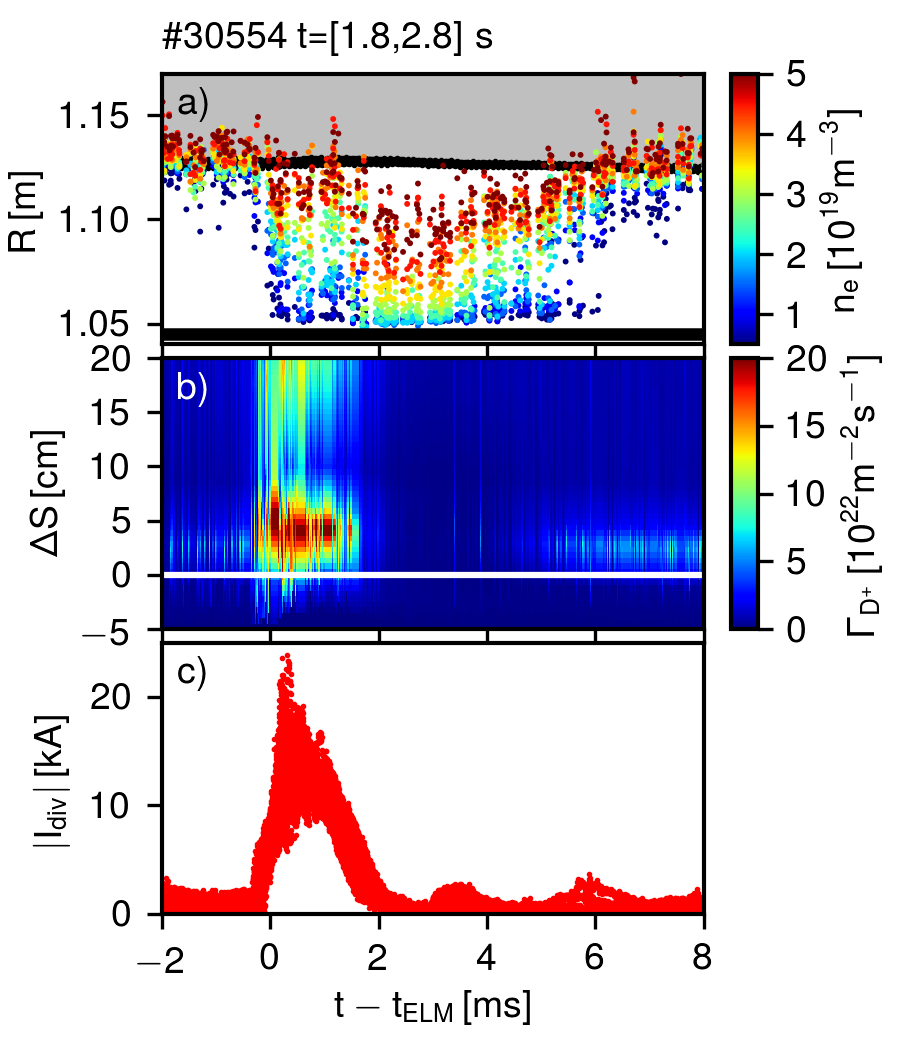
\includegraphics{ssidiv_30554_1_8_2_8_inin.png}
    %\label{fig:rhocomp_30659}
	\caption{HFS.}
	\end{subfigure}
	~
	\begin{subfigure}{3in}
    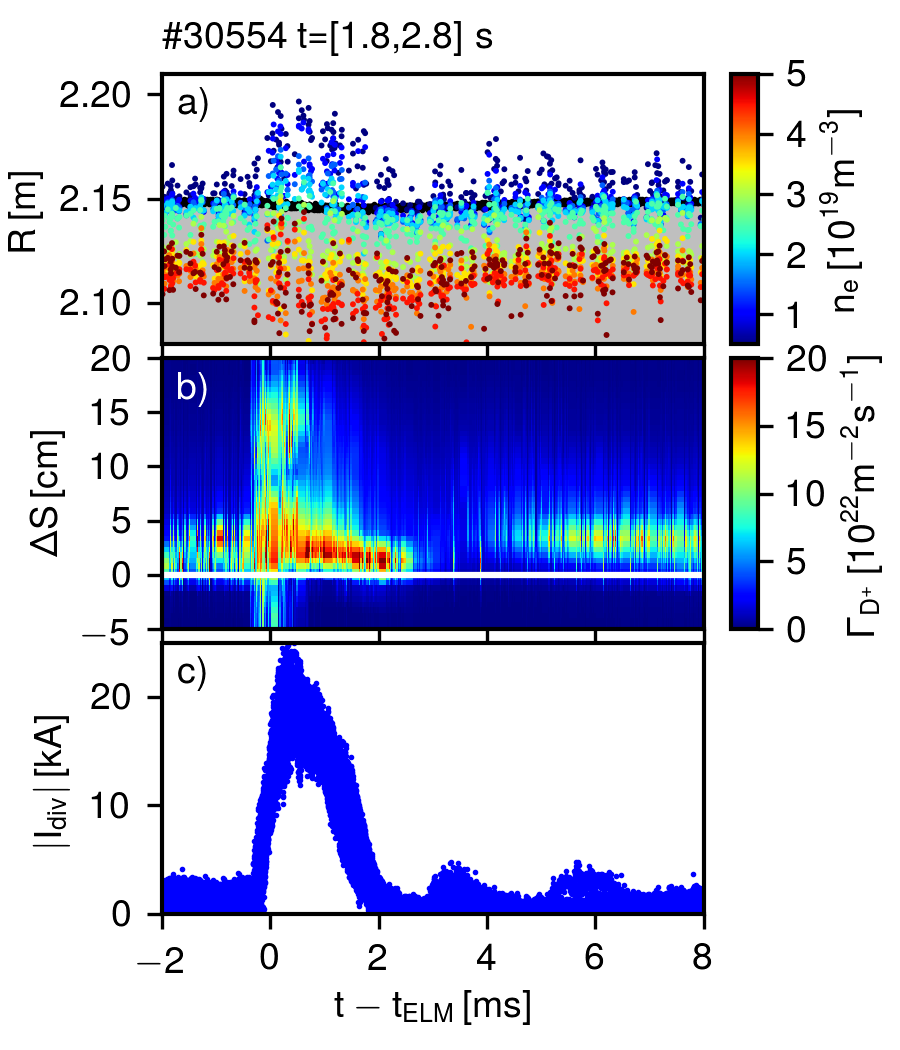
\includegraphics{ssidiv_30554_1_8_2_8_outout.png}
    %\label{fig:rhocomp_30659_hfshd}
	\caption{LFS.}
	\end{subfigure}
	\caption{Phase $I$ of \#30554: Evolution of the conditional averaged density layers from reflectometry at the LFS and HFS during and ELM (a) conditional averaged particle flux to the inner and outer divertor target (b) divertor shunt current (c).}
	\label{fig:elm_30554}
\end{figure}

The LFS density profiles at the midplane exhibit a fast recovery of the midplane density profiles ($2-3\,ms$). About $3-4\,ms$ after the ELM crash an increase in the SOL density is observed that coincides with the changes in the divertor conditions. An increase in the degree of detachment in the outer divertor in a period where the inner target in strongly detached and a HFSHD is present. The increased divertor heat load due to ELMs leads to a temporary re-attachment of the outer divertor during $3-4\,ms$ after the ELM crash with the divertor plasma becoming detach again after this period as indicated by the particle flux measured by the divertor probes. When studying the effect of fuelling and heating power on the inter-ELM profiles, SOL profiles at the midplane have been observed to broaden as detachment is enhanced. The broadening of the SOL density profiles at the midplane after a fast recovery of the profiles may therefore be associated with changes in the divertor conditions.

Previous results\cite{Laggner2018ppcf} show the magnetic activity during the density pedestal recovery is low and consequently the particle flux across the edge is modest. Approximately $3\,ms$ after the ELM onset, medium frequency fluctuations between $30\,kHz$ and $150\,kHz$ set in that are temporally correlated to the stagnation of the density pedestal recovery and the increase in the SOL density.

Conditionally averaged profiles also confirm that the evolution of the density layers at LFS and HFS is significantly different with a HFSHD forming after the ELM crash. As illustrated in figure \ref{fig:elm_30554}, the conditionally averaged particle flux to the divertor is strongly reduced across the entire region explored by the target probes suggesting that the inner target is completely detached. This leads to the formation of a HFSHD extending up to the midplane and resulting in the large SOL densities observed at the HFS by the reflectometry diagnostic. The inner divertor is observed to detach before the outer one and to reach a higher degree of detachment (stronger reduction in $\Gamma_{D^{+}}$ and $T_e$). The HFSHD is induced by the increased particle and heat fluxes to the inner divertor induced by the ELM and is extinguished after the ELM when the energy required to sustain the HFSHD is no longer available and the degree of detachment of the inner divertor is reduced. Our results suggest again that the evolution of the HFS density profiles along the ELM cycle 
is strongly influenced by the divertor conditions.

In the second phase of the discharge, both NBI power and gas fuelling are increased leading to more frequent ELMs. This phase is characterised by the presence of a HFSHD and large HFS/LFS asymmetries in the inter-ELM period as described previously. The larger ELM frequency in this phase allows for improved statistics in the conditional average technique. As displayed in figure \ref{fig:elm_30554_II}, the ELM evolution during this phase is basically very similar to that observed in the first phase but now HFS profiles do not fully recover. The HFSHD exists during the entire inter-ELM period. Density profiles do not become HFS/LFS symmetric at the end of the ELM cycle as observed in the first phase.

The minimum in the LFS SOL density width at $t-t_{ELM} \approx 2-3\,s$ is better defined due to improved statistics and again seems to be correlated with the evolution of the outer target detachment. The temporal evolution of the divertor quantities is also very similar to that in the previous phase with the main difference being that the partially detached phase is now shorter, possibly a consequence of the higher ELM frequency.

\begin{figure}[!hbt]
\centering
	\begin{subfigure}{3in}
    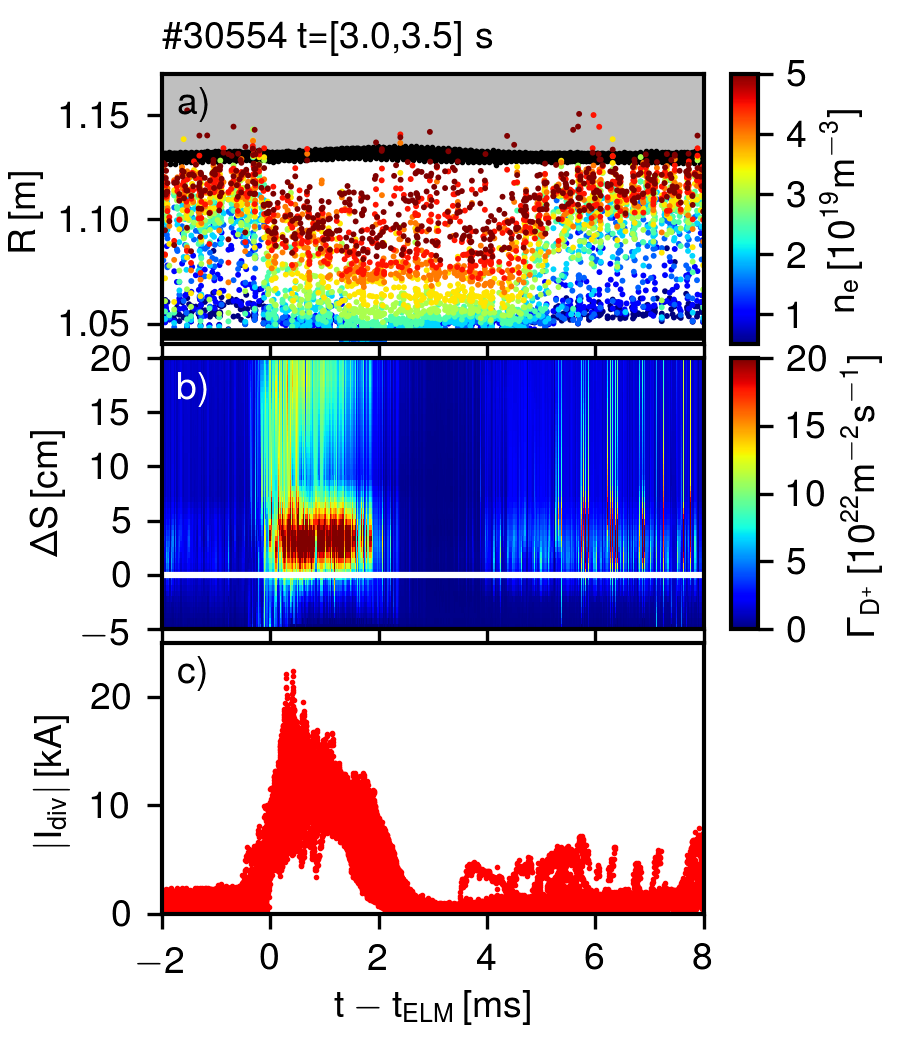
\includegraphics{ssidiv_30554_3_0_3_5_inin.png}
    \label{fig:elm_30554_HFS_II}
	\caption{HFS.}
	\end{subfigure}
	~
	\begin{subfigure}{3in}
    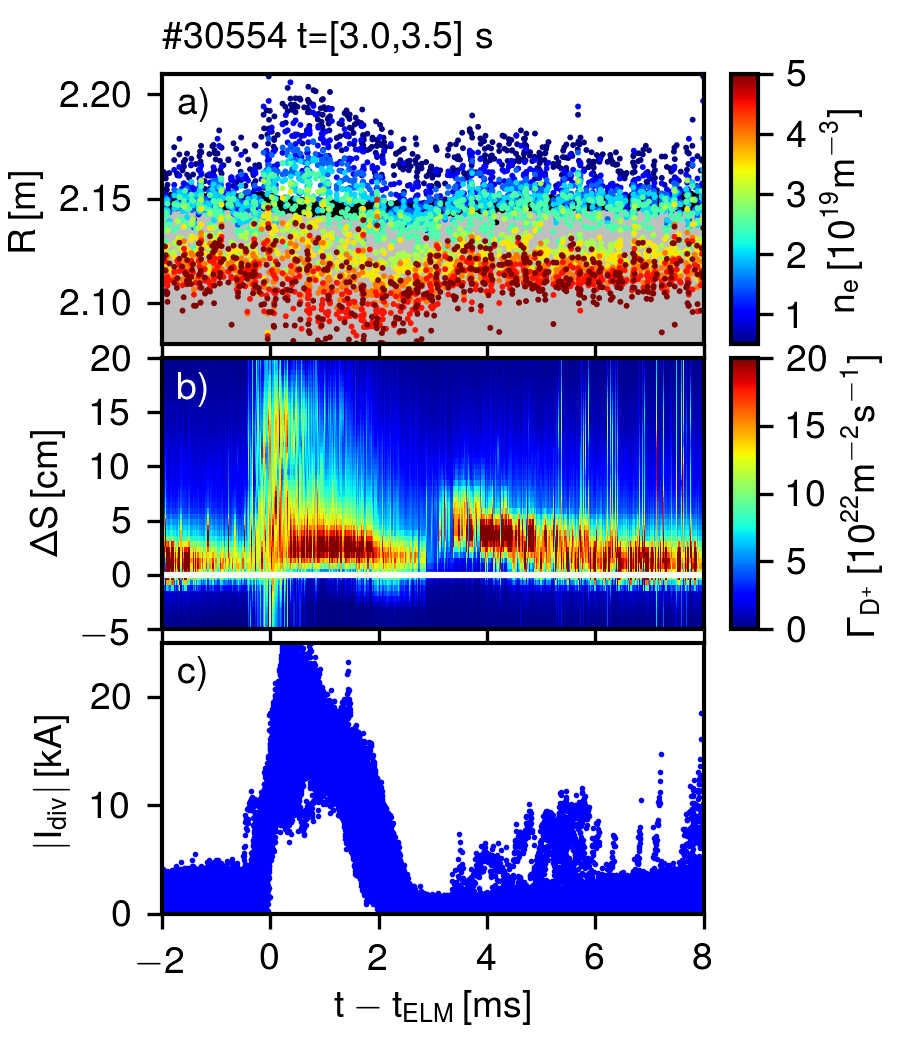
\includegraphics{ssidiv_30554_3_0_3_5_outout.png}
    \label{fig:elm_30554_LFS_II}
	\caption{LFS.}
	\end{subfigure}
	\caption{Phase $II$ of \#30554: Evolution of the conditional averaged density layers from reflectometry at the LFS and HFS during and ELM (a) conditional averaged particle flux to the inner and outer divertor target (b) divertor shunt current (c).}
	\label{fig:elm_30554_II}
\end{figure}

Seeding strongly influences the divertor conditions and therefore it is also expected to modify the evolution of the midplane density during ELMs. When nitrogen seeding is injected in discharge \#30554 (phase III) ELMs are observed to change from type-I to type-III, in line with previous observations at AUG\cite{schneider2014pedestal} and JET\cite{bernert2017power}. The ELM type change impacts reflectometry measurements, as can be seen in figure \ref{fig:elm_30554_III}. The ELM frequency increases to $190\,Hz$ meaning that the duration of the ELM cycle used in the conditional average technique has now to be reduced. However, the evolution of the LFS profiles is generally similar. The drop in the pedestal density is now modest and consequently, the particle flux to the divertor is reduced with respect to that observed in the previous phases. On the contrary, the density evolution at the HFS midplane changes dramatically when seeding is injected. As a result of the reduction in the divertor HFSHD, the HFS/LFS density asymmetry is now smaller with the ELM density perturbation occurring only during a short period below $1\,ms$ with a secondary peak observed about $\approx 2\,ms$ after. The particle flux to the inner target during the ELM crash is now significantly smaller, possibly explaining that no HFSHD is formed after the ELMs during the seeded phase. The inner divertor is completely detached (as indicated by the modest particle flux) but no HFSHD exists at the midplane. This is justified by the seeding promoting detachment while reducing the HFSHD, as the power reaching the inner divertor is reduced by radiation in the SOL.

\begin{figure}[!hbt]
\centering
	\begin{subfigure}{3in}
    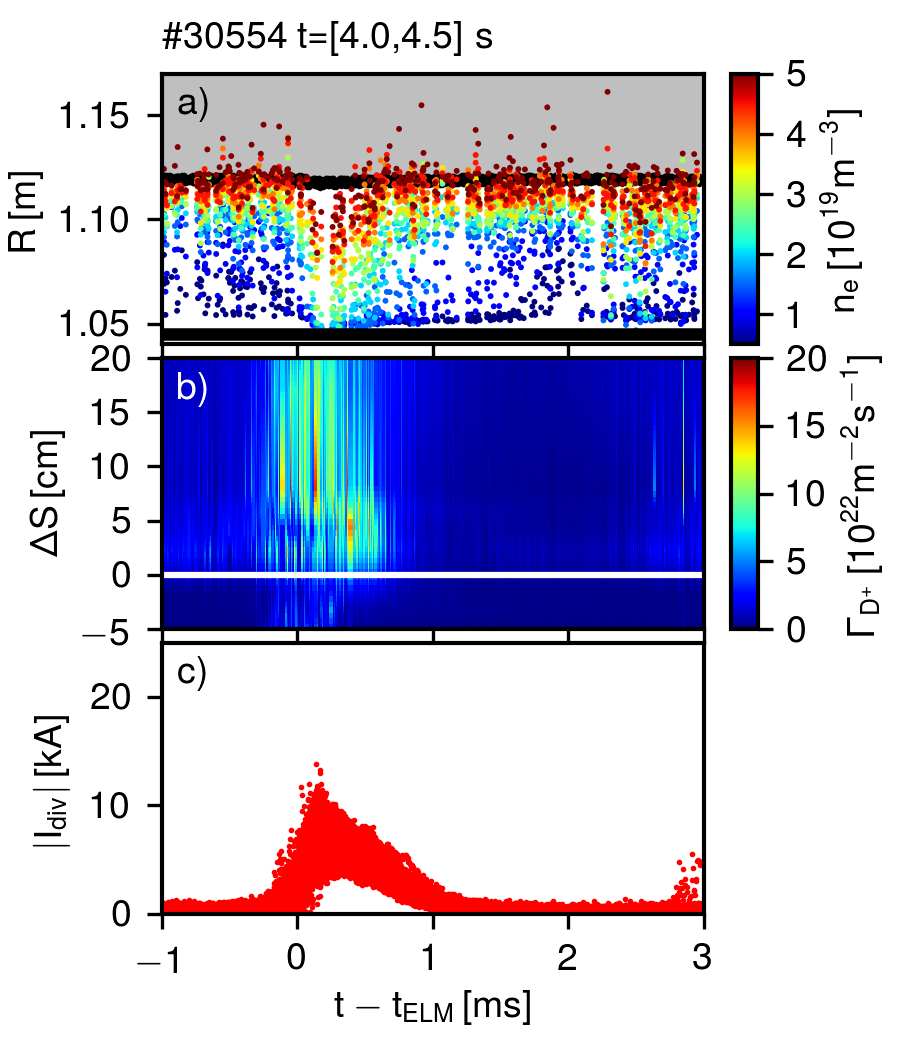
\includegraphics{ssidiv_30554_4_0_4_5_inin.png}
    \label{fig:elm_30554_HFS_III}
	\caption{HFS.}
	\end{subfigure}
	~
	\begin{subfigure}{3in}
    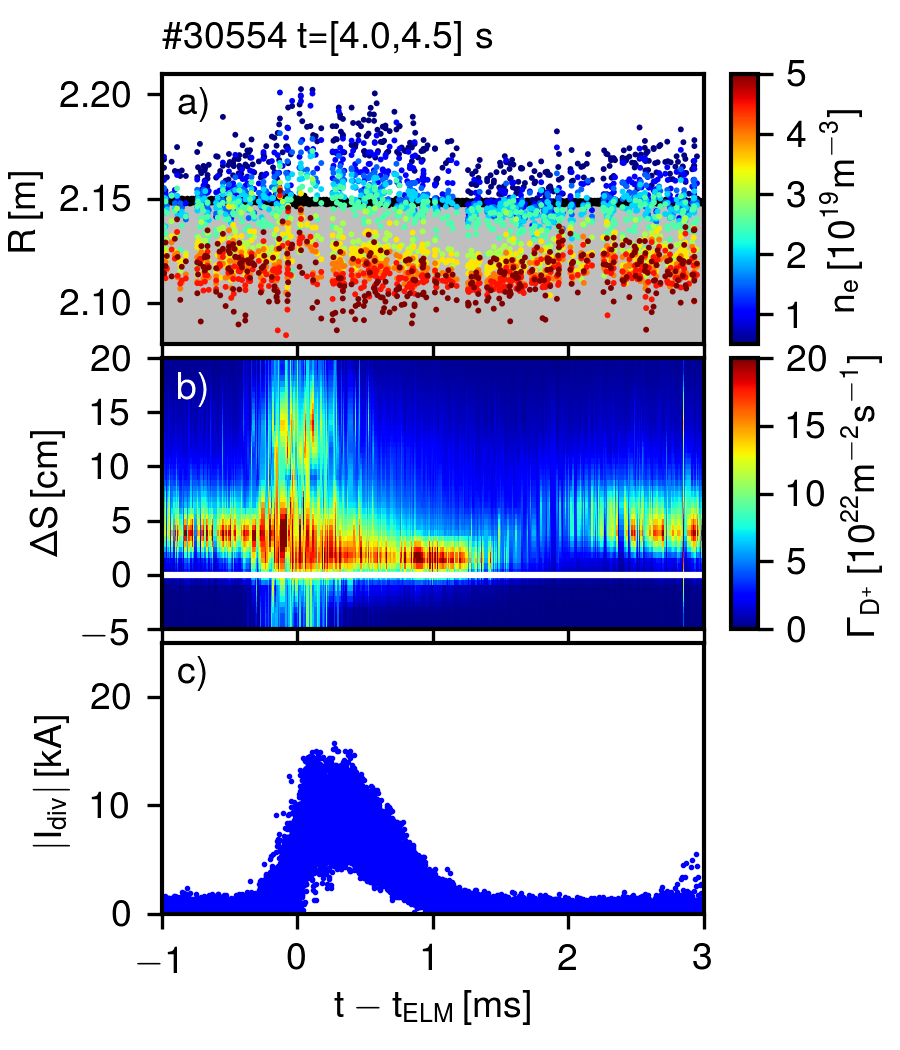
\includegraphics{ssidiv_30554_4_0_4_5_outout.png}
    \label{fig:elm_30554_LFS_III}
	\caption{LFS.}
	\end{subfigure}
	\caption{Phase $III$ of \#30554: Evolution of the conditional averaged density layers from reflectometry at the LFS and HFS during and ELM (a) conditional averaged particle flux to the inner and outer divertor target (b) divertor shunt current (c).}
	\label{fig:elm_30554_III}
\end{figure}

A comprehensive characterisation of the ELM evolution at the midplane and divertor is achieved. The strong effect of the divertor conditions on the SOL density at the midplane is again demonstrated. The most striking result is the observation of a HFSHD at the midplane just after the ELM crash associated with the strong inner divertor detachment. ELMs modify the detachment conditions due to the increased power and particle input to the SOL and in the radiation losses that then reacts back to the midplane SOL parameters and possibly affecting also the pedestal and confinement properties. The LFS density profiles at the midplane were found to exhibit a faster recovery than at the HFS. However, about $3-4\,ms$ after the ELM crash an increase in the LFS SOL density is observed that is most probably related to changes in the divertor conditions. A key element of the study presented here is the ability to measure density profiles at the LFS and HFS during ELMs and relate it to the evolution of the divertor detachment by combining data from several diagnostics.

%%%%%%%%%%%%%%%%%%%%%%%%%%%%%%%%%%%%%%%%%%%%%%%%%%%%%
\section{Discussion and summary}
\label{section:hmodediscussion}

Results presented demonstrate that asymmetries between LFS and HFS density profiles at the midplane also exist in H-mode. In AUG with a tungsten wall, symmetric density profiles are rarely observed, occurring only in low density, low heating power H-modes and preferentially shortly after a machine boronization. Similarly to L-mode discharges, the HFSHD and its effect at the midplane evolves with the detachment state of the inner divertor not existing when this divertor region is fully attached.

Fuelling and heating power have different effects on the density profiles. Fuelling causes an increase in the separatrix density at the LFS in line with \cite{kallenbach2018parameter}, since higher fuelling corresponds to higher pressure at the outer divertor. In addition, fuelling has a rather different effect on the SOL and on the confined region. There is an overall increase in the SOL density with fuelling, particularly near the separatrix while in the confined region the effect is not as pronounced. On the HFS, fuelling also increases the SOL density as a result of the enhancement of the HFSHD. However, no effects are observed at the midplane for the highest fuel rates as profiles are already fully crashed against the inner wall for the density range measured by the reflectometer.

Heating power has a very different effect than fuelling. While only producing a very modest effect on the LFS density profile, changes in heating power greatly affect the HFS density profiles with the HFSHD forming at modest power values. When the NBI heating power is increased from $\mathrm{2.5\,MW}$ (one beam) to $\mathrm{5\,MW}$ (two beams), the HFS density profiles move rapidly into the inner vessel wall, signalling that the HFSHD becomes large enough to manifest itself at the midplane. The exact power threshold needed for the observation of the HFSHD at the midplane has not been established, but it is a relatively low value compared to standard H-mode operation regimes at AUG.

Nitrogen Seeding leads to a reduction of the HFSHD, to an inward shift of the density profile (at both the LFS and HFS) and to a confinement enhancement in agreement with previous observations. A correlation between the reduction of the HFSHD and confinement improvement \cite{Potzel2015,Dunne2017} is thus established. An increase in the fuel rate is also associated with a degradation in confinement and to an increase in the magnitude of the HFSHD, suggesting the existence of a relationship between plasma confinement and the presence of the HFSHD. However, the effect of the heating power does not support the suggested detrimental effect on the HFSHD on confinement. An increase in the heating power leads to a strong enhancement of the HFSHD but also causes an improvement in confinement (although modest, see figure \ref{fig:layers_30733}). Furthermore, the HFSHD is suddenly formed above a certain heating power or fuelling rate threshold without any simultaneous pronounced change observed in confinement.

A comprehensive characterisation of the ELM evolution at the midplane and divertor is performed demonstrating that also during the ELM cycle the divertor conditions have a strong effect on the SOL density at the midplane. The most striking result is the observation of a HFSHD at the midplane just after the ELM crash associated with the strong inner divertor detachment. ELMs modify the detachment conditions due to the increased power and particle input to the SOL that then reacts back to the midplane SOL parameters, particularly at the HFS, possibly affecting also the pedestal and confinement properties. 

\section{Acknowledgements}
This work has been carried out within the framework of the EUROfusion Consortium and has received funding from the Euratom research and training programme 2014-2018 under grant agreement No 633053. IST activities also received financial support from “Funda\c{c}\~ao para a Ci\^encia e Tecnologia” through project UID/FIS/50010/2013 and grant SFRH/BD/87738/2012. The views and opinions expressed herein do not necessarily reflect those of the European Commission.

\bibliographystyle{IEEEtran}
\bibliography{bibliography}

\end{document}
